% das Dokumentenformat
\documentclass[a4paper, 12pt, twppages]{article}

%\usepackage[english, ngerman]{babel}  % <-- f�r deutsche arbeit

% wegen deutschen Umlauten - Details: http://www.golatex.de/usepackagelatin1inputenc-vs-usepackaget1fontenc-t7624.html
\usepackage[T1]{fontenc}
% \usepackage[ansinew]{inputenc} % auf Zeichencodierung der Datei achten! In TeXnicCenter im "Speichern Unter"-Dialog 'ANSI' ausw�hlen.
\usepackage[utf8]{inputenc} % alternative Zeichencodierung 'UTF-8'

%% BIBILOGRAPHY PACKAGE
\usepackage[sorting=none]{biblatex}
\addbibresource{MyReferences.bib}

\usepackage{amsmath}

%% REF PACKAGES
\usepackage{nameref}

%% QUOTING PACKAGE
\usepackage{csquotes}

%% IMAGE PACKAGE
\usepackage{graphicx}

%% PACKAGE FOR THE BACKGROUNDPIC
\usepackage{eso-pic}

%% PACKAGE FOR THE HEADERS AND FOOTERS
\usepackage{fancyhdr}

%% PACKAGE TO INCLUDE A PDF FILE
\usepackage{pdfpages}

%% CAPTIONS
\usepackage{caption}
\usepackage{subcaption}

%% FOOTNOTES
\usepackage[bottom]{footmisc}

%% TABLE PACKAGES
\usepackage{tabularx}
\usepackage{multirow}
\usepackage{booktabs}
\usepackage{array}
\usepackage{float} % prevent table floating to land in next section
\usepackage{colortbl} % for row color
\usepackage{arydshln} % dashed lines
\usepackage[flushleft]{threeparttable}

%% FONT PACKAGES
\usepackage{pifont} % for checkmarks
\usepackage{wasysym} % for checkboxes

%% HYPERLINKS PACKAGE
\usepackage[colorlinks=true, allcolors=black, urlcolor=blue]{hyperref}

\usepackage{tikz}

\tikzset{%
    baseline,
    inner sep=2pt,
    minimum height=12pt,
    rounded corners=2pt  
}

\newcommand{\code}[1]{\mbox{%
    \ttfamily
    \tikz \node[anchor=base,fill=black!12]{#1};%
}}

\newcommand\BackgroundPic{%
\put(0,0){%
\parbox[b][\paperheight]{\paperwidth}{%
\vfill
\centering

\includegraphics[width=\paperwidth,height=\paperheight,keepaspectratio]{background.pdf}%
\vfill
}}}
\fancyhf{}% Clear all headers/footers
\renewcommand{\headrulewidth}{0pt}% No header rule
\renewcommand{\footrulewidth}{0pt}% No footer rule
\fancyfoot[L]{\hspace*{-16mm}
\includegraphics[scale=0.3]{logoDepartment.pdf}}

\newcommand{\importantquote}[1]{
    \medskip
    {
        \setlength{\fboxsep}{.03\columnwidth}
        \noindent
        \colorbox{gray!10}{
            \begin{minipage}
                {\dimexpr\columnwidth-2\fboxsep}
                \raggedright #1
            \end{minipage}
        }
    }
    \medskip
}

\begin{document}

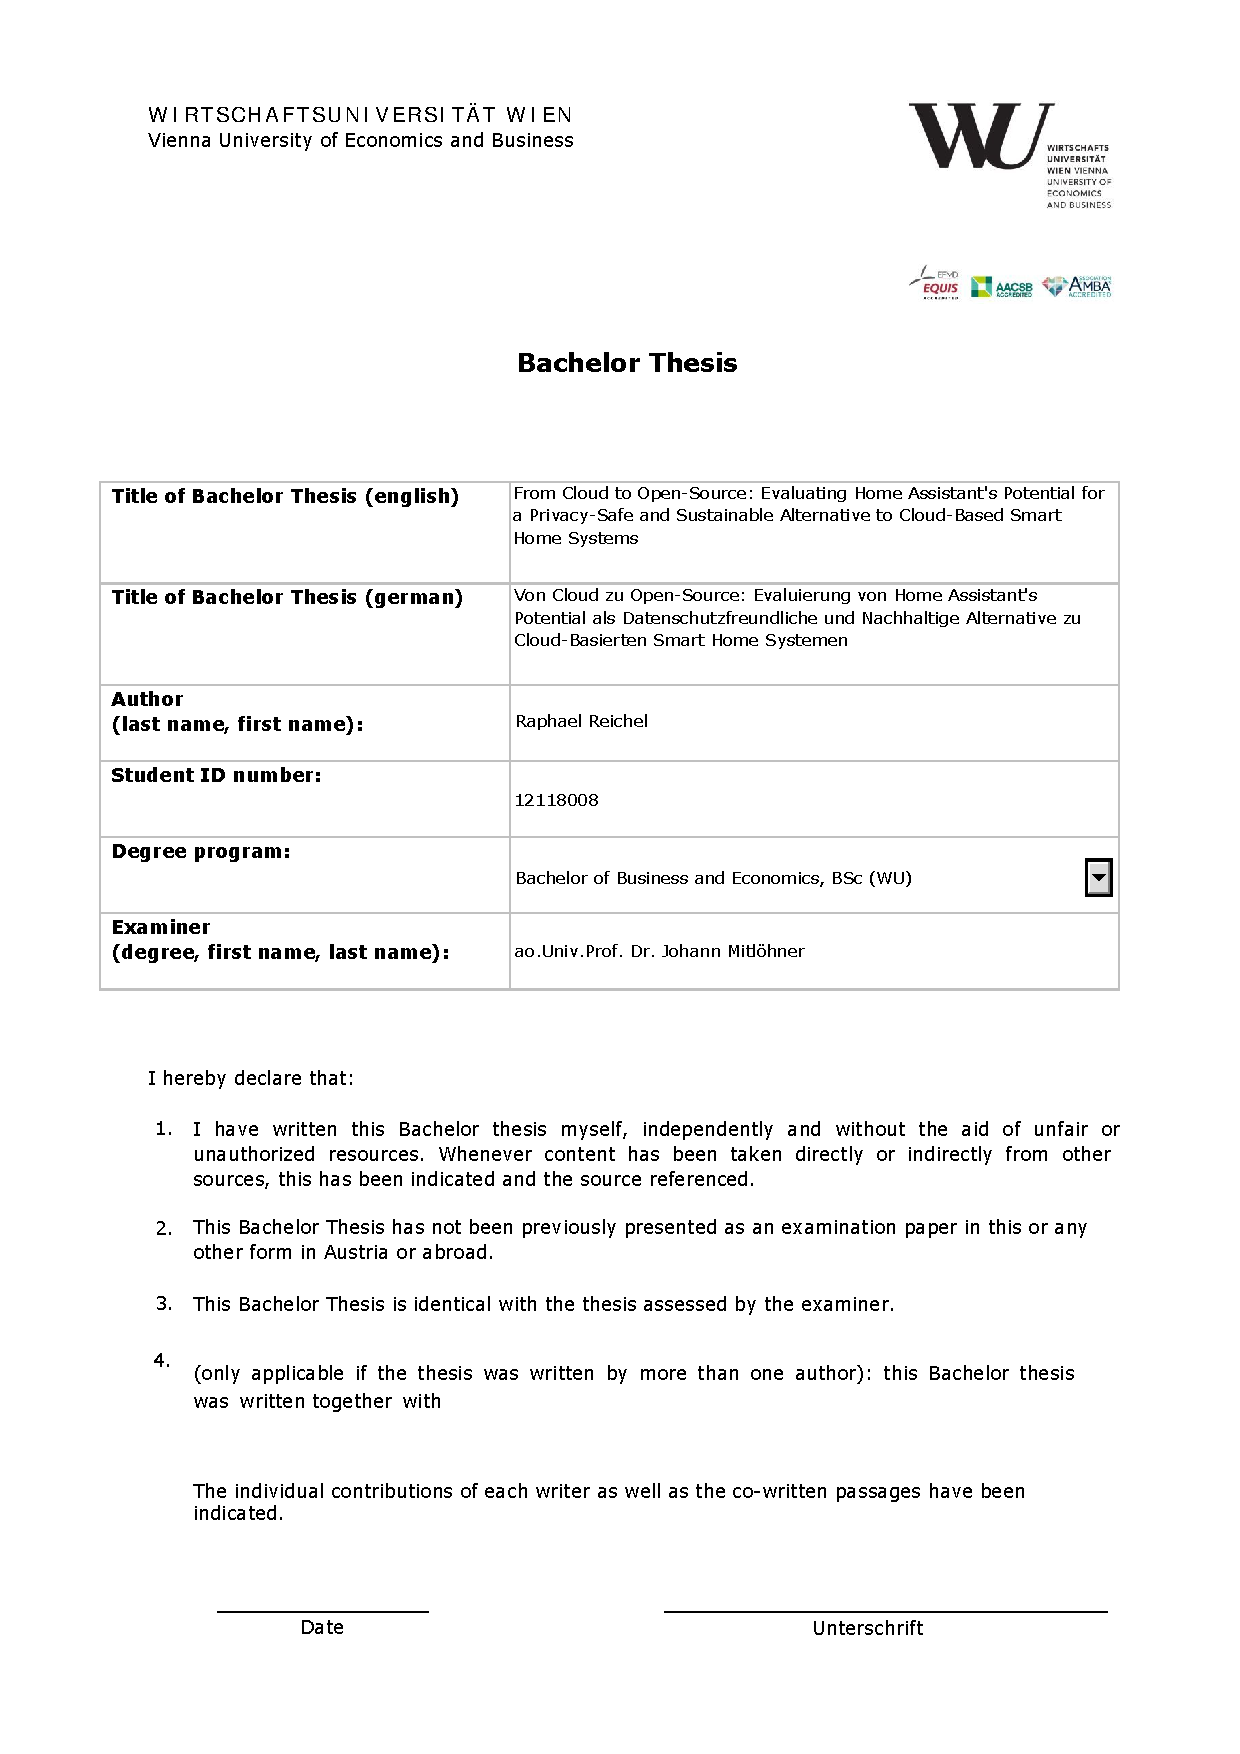
\includepdf[pages={1}]{scan-of-declaration-of-authorship.pdf}
\pagebreak

\AddToShipoutPicture*{\BackgroundPic}
\thispagestyle{fancy}

{\vspace{2cm}~}
{\vspace{2cm}}

%% SELECT BACHELOR OR MASTER THESIS
{\noindent\large Bachelor Thesis}


\vspace{1cm}

%% WRITE THE TITLE OF YOUR WORK
{\noindent\huge\textbf{From Cloud to Open-Source: Evaluating Home Assistant's Potential for a Privacy-Safe and Sustainable Alternative to Cloud-Based Smart Home Systems}}

\bigskip

%% WRITE YOUR NAME, date of birth, Student ID
{\noindent\LARGE Raphael Reichel}

%% WRITE YOUR date of birth, Student ID
\bigskip
{\noindent\small Date of Birth: 19.10.2001}\newline
{\noindent\small Student ID: 12118008}

\bigskip
{\vspace{2cm}}
{\noindent\large {\bf Subject Area:} Information Business}

%% WRITE YOUR Studienkennzahl
\bigskip
{\noindent\large {\bf Studienkennzahl:} UJ 033 561}

\bigskip


%% WRITE THE NAME OF YOUR SUPERVISOR
{\noindent\large {\bf Supervisor:} ao.Univ.Prof. Dr. Johann Mitl\"ohner}

\bigskip

%% WRITE THE DATAE OF SUBMISSION
{\noindent\large {\bf Date of Submission:} TBD}

\bigskip\bigskip\bigskip\bigskip\bigskip\bigskip

{\em\noindent Department of Information Systems \& Operations Management, Vienna University of
Economics and Business, Welthandelsplatz 1, 1020 Vienna, Austria
}


\pagebreak
\tableofcontents
\pagebreak
\listoffigures
\listoftables
\pagebreak


\begin{abstract}
Smart home systems have attracted more and more attention in recent years due to their huge potential to automate home management processes. However, the gained connectivity can potentially endanger the expected privacy within one's home - especially when accounting for the ubiquitous internet access of the modern age. This paper aims to address this cloud-based nature of smart home systems by assessing the current state of this technology, discussing the risk of cloud connections, and proposing a different approach to building a smart home that involves the usage of an open source and locally hosted smart home platform called \textit{Home Assistant}. The paper will start with a brief introduction to the terminology of smart home systems and discuss selected terminologies while focussing on the most commonly adopted smart home platforms. Then, we will examine the imposing risks of smart home devices that are connected to cloud infrastructure and assess a handful of security measures to mitigate associated privacy risks. To emphasize the value proposition of a locally hosted smart home system, a major section of this paper will explore how Home Assistant operates and compare this system to the major competing smart home platforms, as well as highlight important topics for deploying Home Assistant within one's home.
\end{abstract}

\pagebreak


%\renewcommand{\arraystretch}{1.5} % change table row seperation
\setlength{\parskip}{0.556em} % change spacing between paragraphs


%% Section 1 - Introduction

\section{Introduction}

In an era marked by digital transformation, technological advancement did not hold from redefining how we interact with home appliances and thereby continued the trend of digitising every part of our daily life. In the case of the home, this meant integrating small computers into various devices, by which connectivity between previously unrelated appliances emerged, which led to the concept today known as a \textit{Smart Home}.

While undoubtedly yielding many benefits and building unfathomable capabilities for automating home management processes, the gained connectivity can potentially endanger the expected privacy within one's home - especially when accounting for the ubiquitous internet access of the modern age. This risk is amplified by the cloud-based architecture of most traditional smart home systems, which expose home appliances to be controlled from the platform provider's servers. 

This paper aims to address this cloud-based nature of smart home systems by assessing the current state of this technology, discussing the risk of cloud connections, and proposing a different approach to building a smart home that involves the usage of an open source and locally hosted smart home platform called \textit{Home Assistant}.


\subsection{Research question}
The main research question of this paper is:

\importantquote{\textit{How does an alternative to cloud-based smart home systems work and can it improve the privacy of users without limiting their capabilities compared to traditional smart home platforms?} }

\subsection{Research method}
With a view to the aforementioned topics, this paper will start off with a brief introduction to smart home systems and discuss selected terminologies while focusing on the most commonly adopted smart home platforms. We will then later examine the imposing risks of smart home devices that are connected to cloud infrastructure based on literature and case-study reviews, and assess a handful of security measures to mitigate associated privacy risks. The main proposal within this realm will be to deploy \textit{Home Assistant} as a smart home platform and thereby omit the use of cloud connections for controlling smart home appliances altogether. To emphasize the value proposition of this approach, a major section of this paper will explore how Home Assistant operates and compare this system to competing smart home platforms, as well as highlight important topics for deploying Home Assistant within one's home. 

After elaborating this proposal, Home Assistant will be compared to traditional smart home platforms based on its capabilities. Additionally, a small experiment with a few participants will be conducted in order to investigate the entrance barriers for new users who want to deploy Home Assistant on their own. For this the installation and on-boarding process for setting up Home Assistant on a Raspberry Pi will be assessed by the participants. Their experience and feedback will then be used to estimate if this approach of starting with Home Assistant would be appealing to a broader scope of users.

\paragraph{\textit{Open-Access:}}
\label{thesis:github_repo}
This paper, including the used materials, is available at this public github repository: \href{https://github.com/dir-rafa/Bachelor-thesis-Home-Assistant}{https://github.com/dir-rafa/Bachelor-thesis-Home-Assistant}

\newpage

%% Section 2 - Introduction Smart Home

\section{Smart Home Systems}
A \textit{Smart Home System} is the superset of connected devices and technologies that represent the physical and logical subtleties that make up the \textit{Smart Home}, but is most commonly used as a synonym for the \textit{Smart Home Platform} that handles communication between multiple devices and hosts the respective user interface.
This terminologies do not really refer to the same concepts, since controlling devices via multiple platforms could have some benefits, e.g. different household residents want to use their respective Android or iOS native smart home platforms, but separating devices into multiple systems and therefore isolating them from communicating with another, will most often not be desirable.

A major point of differentiation of smart home systems is the medium that connects devices together \cite{ReviewOfSmartHomes-6177682}. While many alternatives exists for wireless systems \cite{ReviewOfSmartHomes-6177682}, \textit{KNX} dominates the market for wired systems \cite{BertkoChris2017HSH:}. Since the latter must be planned in advance and requires physical connections between devices, they are more expensive than wireless systems and are only deployable within the scope of a major renovation or construction of a new building \cite{BertkoChris2017HSH:}. Therefore, wireless systems are particularly interesting for homeowners who want to upgrade their existing home to a smart home. Moreover, this approach has the benefit that expanding the system is easier to accomplish as no new wires are required. For this reason we will focus on wireless systems when discussing smart home platforms, but first of all we will explore what a smart home is.

\subsection{What is a Smart Home?}
At its core a \textit{Smart Home} is an interconnected network of home appliances that enables the home owner to perform actions that they would not be able to perform, in a comparative form, without the ability of the devices to communicate with each other. This does not necessarily require the user to perform manual actions, such as operating a light switch, but rather means that some trigger (like a switch or a sensor) can have an effect on a wider scope of appliances than itself is physically connected with. A common example for this is a self-regulating heating system, where temperature sensors control when a room needs to be heated, but the system is interrupted by smart contact sensors if the windows are opened \cite{BertkoChris2017HSH:}. The same system can be later expanded by setting a time trigger to warm up the bathroom before a resident gets up in the morning \cite{Tuohy2023SHP}.

For this reason smart homes are often referred to as "intelligent living"\cite{BertkoChris2017HSH:}, since they enable home electronics to be controlled from a central hub and automate processes to perform a set of actions that would otherwise require multiple interactions of the user \cite{BertkoChris2017HSH:}. This central hub is a core pillar of most smart homes and influences the set of capabilities the homeowner has to their disposal to create these action-sets. A core difference to conventional control systems is the aforementioned \textbf{expandability} of smart homes, meaning that additional devices or sensors can be easily added at any given time.

In addition to automating actions, this also enables the homeowner to repurpose their devices to perform tasks they were not supposed to perform initially. Given that some subset of devices, which typically are associated to be used only by residents (e.g. TVs or lights), communicate within this network, clever use of automations based on triggers like the current time can be used to create a simple presence simulation \cite{BertkoChris2017HSH:}, which creates the illusion of activity within a home and, therefore, fools outsiders to believe that the home would be occupied at the moment.

This combination of capabilities shows the \textbf{emergent property} of smart homes, meaning that new utility can be created by re-contextualising the existing environment and leveraging the individual feature-sets of devices. Consumers perceive this property as the modularity of smart home systems, which has a great influence on the perception of the value of smart home \cite{TangRuiyang2021SoPE}.

In some sense a Smart Home can be viewed as the "[...] natural evolution of our homes. A smart home is not fundamentally different from a 'regular' home - it is just the improvement of one."\cite{Tuohy2023SH}. In fact, smart homes are not a new technology or a sudden technological development. We have been putting computers into home appliances for more than a decade \cite{Tuohy2023SH} and thus laying the foundation for the interconnected world in which we live today. What started with devices such as light bulbs, outlets, or thermostats led to the development of doorbells, locks, and vacuums, all controllable from a smartphone \cite{Tuohy2023SH}.

Like the uniqueness of physical houses, two distinct smart homes will always differ from each other. Although they may share certain properties, one should not imagine building a smart home as a normed operation. While a house must have an entrance and probably will have some windows, a smart home must have a common communication protocol and likely will have some form of user-interaction interface, but the physical location and material of that house windows will be determined by the preferences of the homeowner. Likewise the preferences for the visual representation of the user interface, or deployed technologies, will be different on a home to home basis depending on the requirements and needs of the homeowner. Therefore, smart homes can fulfil different purposes and \textbf{ operate at different levels of complexity} according to the preferences, interests, and technical proficiency of their owner.

\subsection{Smart Home Platforms} \label{sec:Smart Home Platforms}
The \textit{Smart Home Platform} is a software framework that provides services to a smart home that enables the execution of actions with higher levels of complexity such as automations, serves as an organisational layer of abstraction (e.g. to group devices together), and acts as a central hub for managing smart devices. One of its core tasks is to handle communication between devices that use different communication protocols \cite{ReviewOfSmartHomes-6177682} or follow different specifications from different manufacturers \cite{Tuohy2023SHP}. Moreover, smart home platforms often provide a graphical user interface in the form of an smartphone-app or web interface for controlling devices and hosts some notification system to inform the user about changes or alerts. The organisation of devices is most often done by grouping them by their location into \textit{rooms} that act as a digital counterpart of the physical house \cite{BertkoChris2017HSH:}.

The most popular smart home platforms for consumers are developed by large tech companies \cite{Tuohy2023SHP} and are well known for their simple installation and easy integration of popular devices. Without particular order those \textit{mainstream smart home platforms} are:
\begin{itemize}
    \item \textbf{Amazon Alexa} - developed by Amazon
    \item \textbf{Apple Home} - developed by Apple
    \item \textbf{Google Home} - developed by Alphabet
    \item \textbf{Samsung SmartThings} - developed by Samsung
\end{itemize}

Most smart home platforms require a physical hardware component such as a \textit{hub} \cite{BertkoChris2017HSH:} that can host these services, but many manufacturers combine this with some other type of appliance such as a smart speaker \cite{Tuohy2023SHP}, but sometimes they are just small pucks that sit in an outlet somewhere in a home \cite{Tuohy2023SHH}. In any case, they act as the brain of the smart home platform and are essential for their operation.

In addition, hubs commonly incorporate radios for various wireless technologies that are required for local communication with devices \cite{Tuohy2023SHH}. Local connectivity means that a smart home could be operated without a cloud connection and therefore stay operational in the event of an internet outage. However, not every smart home platform is equally independent from their manufacturers cloud. Especially voice assistants tend to be rendered useless without a cloud connection. Although some basic voice commands will most often work offline, more complex tasks require an active Internet connection. The importance of cloud connectivity for e.g. Alexa is apparent on their support site. The word "cloud" is mentioned 76 times in their roughly 18-page long FAQ-section about the operations of their voice assistant \cite{AmazonAlexaFAQ}.

A common property of three of the four above-listed smart home platforms (with Alexa being the exception) is that they are developed by companies which also develop smartphones. They are also natively installed on those mobile devices. Although this in itself may not be significant for their success reasons, there might be an incentive for users to deploy the smart home platform that is developed by their phone manufacturer.

Besides aforementioned platforms, there are many other alternatives that are direct competitors or have a focus on specific use cases. \textit{Home Assistant} is one of them and will be assessed in detail in section \ref{sec:Home Assistant}.

The choice of platform also determines the smart home community in which a user is likely to participate, as they may want to share their experiences with other consumers. This community influences the user's perceived value of smart home devices by creating social value through inter-consumer cooperation efforts \cite{TangRuiyang2021SoPE}.


\subsection{Considerations when starting with Smart Home}
It should be clear by now that building a smart home is not an easy task. Many decisions made along the way can influence the user's capabilities in the future, and likewise the environment in a home can change drastically. Even third parties can affect a smart home system. The devices deployed today will likely receive updates throughout the years, which can benefit the user, but can also change the software in such a way that the current way of operations has to be adapted.

One of the most important initial considerations will be to decide \textbf{which platform to use} \cite{Tuohy2023SHP}, since this will determine \textit{how one interacts} with the smart home and \textit{what technologies it can support}.

At this point users have a wide array of options, but many tend to deploy one of the four aforementioned mainstream platforms \cite{Tuohy2023SHP}. A deterministic for this decision could be that \textit{users favor to build upon devices and technologies that they are currently using}. The already made argument that the users smartphone may influences their choice of smart home platform would support this hypothesis and leaning towards the platform of a manufacturer whose other devices (e.g. smart speakers, smart tv system, etc.) already provide value to the user, sounds plausible too. Therefore the owned devices may well be a good guide for what smart home platform is a good fit for starting a smart home \cite{Tuohy2023SHP}.

In addition, the user has to ask themselves \textbf{what features they need} their smart home to have \cite{Tuohy2023SHP}. This ultimately influences the choice of their platform too. While Apple Home is known for their secure video platform (\textit{Homekit Secure Video}) that processes footage of surveillance cameras locally before encrypting and storing them in the cloud \cite{Kastrenakes2019HKSC}, Samsung Smart Things offers an energy management system that can help users to cut down on their electricity usage \cite{Tuohy2023SHP}\cite{SamsungSmartThingsEnergy}. Similarly, Amazon Alexa uses artificial intelligence to help users in their daily lives with suggestions based on their typical behaviour \cite{Liao2018AH}.

Above all \textbf{users have to trust a platform} and thus the manufacturer who is developing the platform of their choice, since they are likely dependent on the cloud infrastructure of the providers for e.g. processing voice requests (see section \ref{sec:Smart Home Platforms}), store data like video footage \cite{Kastrenakes2019HKSC} or analyse user data to give them insight into their behaviour \cite{Liao2018AH} and energy consumption \cite{SamsungSmartThingsEnergy}.

However, \cite{ZhengSerena2018UPoS} shows that users seem to priorities convenience and connectivity when selecting smart home devices. Privacy concerns are infrequent among users, as they typically just assume that their privacy is protected by the manufacturers. This decision is rarely based on evidence, but leads users to buy into potential privacy risks as machine learning can reveal sensitive information from usage data \cite{ZhengSerena2018UPoS}.

But what if trusting manufacturers with protecting privacy data in the cloud would not be necessary at all? The scope of this paper is to introduce an alternative to these cloud-based smart home platforms: \textit{Home Assistant}. Therefore we will make the assumption that \textit{users do not want to trust manufacturers with their data} and explore if smart home can work without a cloud that is operated by third parties. In order to examine how smart home devices can endanger the privacy and security of users, the next major section will assess associated risks that cloud-based devices may impose on smart home systems and their users.

\newpage

%% Section 3 - Risk Analysis

\section{Risks of Cloud-Based Smart Home Devices}
Information security (InfoSec) is a common foundation in many it-systems to ensure basic security requirements. Likewise, smart home systems should comply with these principles and aim to ensure \textbf{Confidentiality}, \textbf{Integrity} and \textbf{Availability} of services and data within the smart home \cite{SecurityConsiderations-7354752}. Those requirements are reasonable to satisfy since devices are likely to be exposed to various threats from inside and outside the home network given that they often will have internet access \cite{SecurityConsiderations-7354752}.

%In the context of smart homes

This section will focus on curated cases where cloud-based smart home devices endanger these foundational principles. Cloud connections undoubtedly can improve the convenience of smart home systems, but users have to consider potential drawbacks when deploying third-party services.

\subsection{Implications of Public Server Connections}
\label{sec:implications-server-connections}
Granting smart appliances internet access enables them to establish a connection to external services, such as their manufacturers cloud. Although this communication may be desired by the user for receiving external information, these devices can also deliver their gathered information to outside services. Since some devices collect sensitive data, some users may therefore have concerns about the deployment of smart home devices within their home \cite{ImprovingPrivacyControl-8514198}. This perceived privacy encroachment is often enhanced by nonintuitive and nontransparent device configuration options. Only a few smart home devices allow one to customise the storage locations of collected data and frequently deploy \textit{Zero-Conf configuration processes}, where the manufacturer enforces default security and privacy configurations \cite{ImprovingPrivacyControl-8514198}. Moreover all of this has to be configured on a device-on-device basis what makes configuring large deployments time consuming when a user wants to deviating from the default configuration.

An often overlooked risk of cloud-dependent smart home devices is the eventuality that the device's manufacturer could turn off their servers any day. This exact scenario is what happened in 2016 to users of a smart home hub made by \textit{Revolv} which had been acquired by \textit{Nest}, a company operated by Google. They decided to drop their support of Revolv products which effectively turned their devices into e-waste overnight \cite{Proctor2020BH}. Revolv's FAQ page declared that all services will be terminated, their app will no longer open, and the hub will no longer be operational (see figure \ref{fig:Revolv-FAQ-Services}) \cite{Gilbert2016Nest}.

\begin{figure}[H]
    \centering
    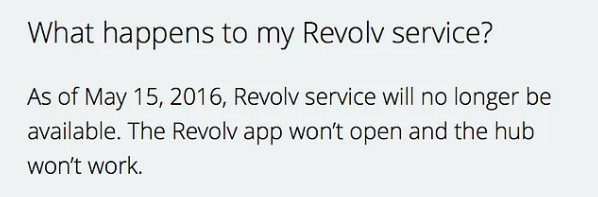
\includegraphics[width=.65\linewidth]{Bachelorarbeit/img/revolv-faq-service.png}
    \caption{Revolv FAQ about their services \cite{Gilbert2016Nest}}
    \label{fig:Revolv-FAQ-Services}
\end{figure}

A Revolv user named Arlo wrote an article about his experience on \textit{Medium} and said: \blockquote{\textit{On May 15th, my house will stop working. My landscape lighting will stop turning on and off, my security lights will stop reacting to motion, and my home made vacation burglar deterrent will stop working. This is a conscious intentional decision by Google/Nest.} \cite{Gilbert2016Nest}}

This case shows the potential dangers of cloud dependency in smart home systems for availability and longevity of devices. Not every device will stop working once they can not make a connection with their manufacturers cloud, but the services related to it will terminate overnight once the company pulls the plug of their servers. 

A more recent example of this happened in 2024 when \textit{Spotify} decided to discontinue \textit{Car Thing}, a product designed to control Spotify in the car that was produced in 2022. Their FAQ site now suggests to simply dispose of the product (see figure \ref{fig:Spotify-FAQ-CarThing}) \cite{OpenHomeBlog_CloudProducts}.

\begin{figure}[H]
    \centering
    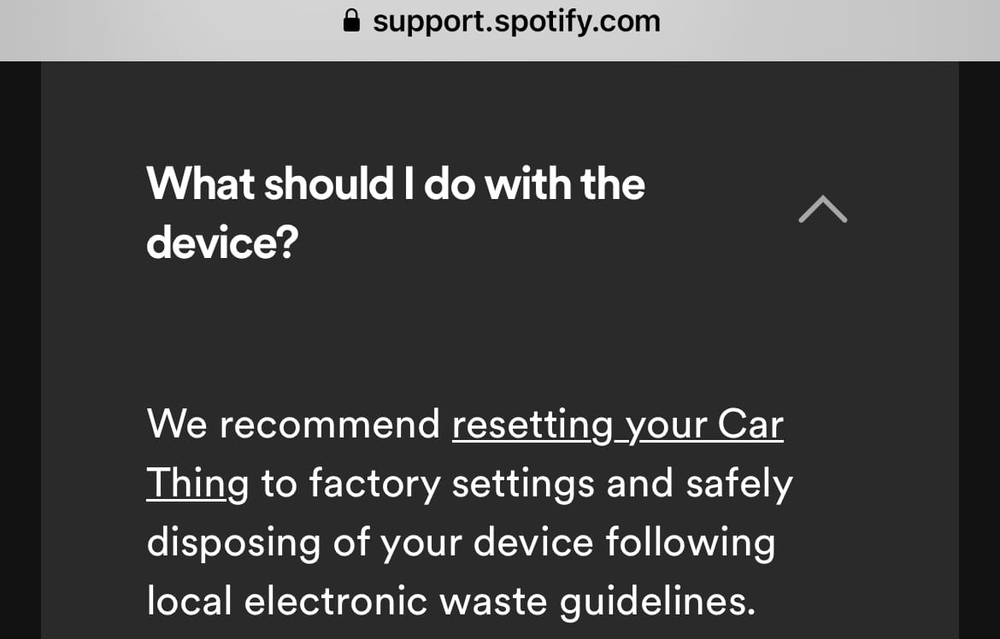
\includegraphics[width=.65\linewidth]{Bachelorarbeit/img/spotify-throw-away.png}
    \caption{Spotify FAQ for Car Thing \cite{OpenHomeBlog_CloudProducts}}
    \label{fig:Spotify-FAQ-CarThing}
\end{figure}

Additionally, the aforementioned consequences would also apply if the user's Internet connection goes down or the manufacturer faces temporary connection issues \cite{BertkoChris2017HSH:}. Therefore, users should carefully consider if they want to blindly trust any company they deploy devices from within their smart home.

\subsection{Unauthorized Access to Smart Home Devices}
Features like cloud storage might be perceived as convenient by smart home users, but imply that the collected data is not physically owned by them. Depending on the nature of the stored data and the technologies used to secure it this could have more or less severe consequences.

The video doorbell and surveillance camera company \textit{Ring}, owned by Amazon, has been known for sharing video footage with law enforcement agencies in the United States. Ring introduced various systems where users were able to respond on public or private police requests where they could provide their recordings to help investigations of crimes near their location \cite{Kaur2024Ring}. While this service was build on the consent of the product owner, Ring also provided video footage on their own in "rare occasions" if police indicated an emergency and therefore Ring disclosed the private recordings of affected users without the law enforcement agencies requiring a warrant \cite{Kaur2024Ring}. This shows that depending on how a company stores their user data, they might be able to access this data on their own initiative. This case also shows that they might be able to give third parties access to a user's data without their knowledge or consent.

Ring is not the only security camera company that is known to comply with these types of emergency disclosure requests. Google, the company behind \textit{Nest} stated within an interview with \textit{The Verge} that based on their terms of service they would be allowed to send data to authorities without a warrant or consent of the user \cite{Clark2022Nest}.

However, not every company can or will comply with this requests. Apple also offers to store user video footage on their servers, but uses end-to-end encryption with their \textit{Homekit Secure Video} service \cite{Kastrenakes2019HKSC} and therefore claims not even to be able to comply with these requests due to the technical implications of their encryption technique \cite{Clark2022Nest}.

\subsection{Eavesdropping by Voice Assistants}
Smart home voice assistants are known to have many attack vectors and various privacy and security concerns as shown in \cite{SHPA-10.1145/3412383}. While all of them should be taken seriously, this section will focus on the most immediate and user-centred privacy issue at hand that involves cloud-connectivity.

Voice Assistants offer a unique way of interacting with smart home devices with the capability to respond to voice commands, allowing the user a hands-free operation of their smart home \cite{SHPA-10.1145/3412383}. To achieve this they wait for a predefined \textit{wake-word} and record what the user says after that. This recording is then sent to a compute node which analysis the data using \textit{Natural Language Processing} for identifying the users intent that eventually can be used as input for an artificial intelligence to issue following actions \cite{SHPA-10.1145/3412383}.

This process involves \textbf{two critical points of failure} that can endanger the privacy of users. First as stated in \cite{SHPA-10.1145/3412383} the voice assistant is "\textit{Always On, Always Listening}". The wake-word can be said accidentally or falsely recognised by the device due to any other phonetically similar word during an unrelated conversation. This would trigger the voice assistant to record the following conversation, which consequently \textit{will then be uploaded to the Internet} \cite{SHPA-10.1145/3412383}. This is because the second critical point of failure is the involvement of the manufacturers cloud. Almost all voice assistants are Internet-based systems that process most of their voice processing in their manufacturers cloud, where, moreover, they store transcripts or recording for improving their model. In fact, only the wake-word is recognised locally on the device \cite{SHPA-10.1145/3412383}\cite{BertkoChris2017HSH:}.

The implications of this cloud communication and storage of user data were already discussed in the previous sections, and similar concerns arise when reviewing incidents related to voice assistants. In 2018 one specific case was covered widely in the media where Amazon's \textit{Alexa} sent a recording of private conversations to a random contact of a user without being explicitly asked to do so \cite{Horton2018AlexaRecordsConversation}. A representative of Amazon explained: "Echo woke up due to a word in background conversation sounding like 'Alexa.' Then, the subsequent conversation was heard as a 'send message' request. [...]" \cite{Horton2018AlexaRecordsConversation}. The company then declared the case as a malfunction. Later in the same year, an Amazon customer received 1,700 audio files that contained recordings of strangers' voice requests made to Alexa. The information within the audio files together with a Facebook and Twitter search was enough to identify the stranger, who had not been contacted about the incident by Amazon before gaining public attention \cite{Ingber2018AlexaAudioFiles}. Although those two cases are rare incidents, they show what data voice assistants collect and possibly can expose about their users.


%% Section 4 - Security Measurements

\section{Securing a Smart Home against Cloud-Risks}
This section will discuss three approaches to reduce user exposure to some of the potential negative consciences of cloud-based smart home devices that were highlighted above.

\subsection{Avoiding Cloud Connections}
One straight forward approach how a user can reduce cloud connections within their smart home is to deactivate cloud services in the settings of their deployed devices. If it stays operational and the user experiences no drawbacks then the cloud service was optional to begin with and therefore can be easily disabled. This is the case for services like \textit{out of home control}, where users can access their smart home from outside their residential home network. Deactivating those will only impact the user when they need to control the specific device remotely and have no alternative means of control through another smart home controller. 

While some manufacturers, like \textit{Bosch} \cite{BoschHelpSmartController} or \textit{Shelly} \cite{ShellySmartControlApp}, who both develop various smart home devices for controlling lights, shutters and indoor climate controller, will allow users to disconnect their devices from their cloud services, others like \textit{Philips Hue} will have mandatory cloud connections \cite{Tuohy2023PhiliphHue}. This shows that combating cloud connections as an afterthought could potentially be troublesome, as not every device will allow the user to disconnect from all cloud services entirely.

Therefore, considering cloud connections before purchasing a fleet of smart home devices will yield better results to limit the overall amount of outside connections. Carefully selecting the smart home device manufacturers that the user trusts will also help avoid future frustrations in this domain. Moreover, it could be wise to consider if any device without a local API would even be worth deploying within a smart home, since local control will at least work for the entirety of the device's lifespan. 

\subsection{IoT Network Security}
A common security approach to control the network traffic of devices is to establish VLANs that essentially operate as separated virtual networks and to implement powerful firewall rules to block unwanted traffic. Those techniques are also suitable for smart homes to protect against various threats \cite{SH-NetworkSecurity-9990734}. Furthermore, network segmentation can be used to block cloud connections on the network layer by setting up an \textit{IoT-VLAN} and configuring separate firewall rules for this segment. Smart home devices can be placed on this network, which then can be used not only to isolate devices from the Internet, but also to protect personal devices or sensitive data on the network from being accessed by IoT devices \cite{BMI-SmartHomeSecurity}. This can also be taken one step further by deploying \textit{Private VLANs} that isolate devices completely from one another, so that all traffic must go through the router \cite{SH-NetworkSecurity-9990734}.

Some modern routers provide the option to easily configure a separate WiFi network to integrate only IoT devices \cite{BMI-SmartHomeSecurity}. Alternatively, the \textit{Guest-WiFi} often serves a similar purpose. However, setting up firewall rules to block smart home devices from connecting to their cloud server requires some technical knowledge from the user. Therefore, network security can be difficult for smart home novices to configure.

Even so, blocking network traffic can be very effective when devices offer a local API but do not allow the user to deactivate all cloud connections.

\subsection{Matter Protocol}
The \textit{Matter} Protocol is an open-source connectivity standard developed by the \textit{connectivity standards alliance} for controlling smart home devices \cite{Matter-Security&Privacy}. It is supported by major industry leaders such as Apple, Google, Amazon and Samsung with the goal of creating an ecosystem where smart home devices can communicate with another regardless of their manufacturer \cite{Matter-10288747}. It has been designed with state of the art security and privacy principles in mind which among others require Matter devices to be fully controllable locally \cite{Matter-Security&Privacy}.

While Matter does not rule out cloud connections \cite{Matter-Security&Privacy} it ensures that its devices will still be operational in the event that a manufacturer shuts down their cloud services. Therefore, endorsing the Matter protocol elevates the potential danger to end with abandoned devices like in the case of Revolv or Spotify presented in section \ref{sec:implications-server-connections}.

\newpage

%% Section 5 - Home Assistant

\section{Alternative to cloud-based Smart Home Systems: Home Assistant} \label{sec:Home Assistant}
\textit{Home Asssitant} is a community-driven \textbf{open source} smart home platform that puts \textbf{local control} and \textbf{privacy first}. It has been designed to run on local servers and mini computers like the \href{https://www.raspberrypi.com/}{Raspberry PI}\footnote{https://www.raspberrypi.com/} without depending on the cloud \cite{HomeAssistant_Startpage}.

The project was started by Paulus Schoutsen in 2013 with the initial aim to take greater control of the Philips Hue devices that he had purchased at that time. Over the course of the coming years and with the help of mainly volunteer contributors, Home Assistant has grown to become one of the leading smart home platforms \cite{OpenHomeFoundation_About} and the most widely used home automation system for DIY enthusiasts.

Home Assistants fundamental vision is to build a smart home that protects the values of what they call \textbf{The Open Home}:

\importantquote{
    The Open Home is about \textbf{privacy}, \textbf{choice} and \textbf{sustainability}. [...]\\[1.5ex]
    \textbf{Privacy} for the Open Home means that devices need to work locally. No one else needs to know if you turn on a light bulb or change the thermostat. \\ It is okay for a product to offer a cloud connection, but it should be extra and opt-in. [...]\\[1ex]
    \textbf{Choice} for the Open Home means that devices need to make the gathered data available through local APIs. This avoids vendor lock-in and allows users to create their own smart home with devices from different manufacturers. [...]\\[1ex]
    \textbf{Sustainability} for the Open Home means that devices are designed and built to keep working and use as little energy as possible. Not just this year, but for the next decade. If they outlive their original purpose, they should be able to be reused or repurposed for something else. [...]\\[1.5ex]
    
    --- Paulus Schoutsen about \textit{The Open Home} \cite{HomeAssistant_Blog2021TheOpenHome}
}

In 2024 the core group of developers decided to protect and codify their ideals of the Open Home and created the \textit{Open Home Foundation}, a non-profit organisation that acts as a formal home for open source projects so that they are protected from future buyouts and abandonment. The Open Home Foundation holds ownership of more than 240 smart home projects, standards, drivers, and libraries. Home Assistant being one of them \cite{OpenHomeFoundation_About}.

All of this is funded by the for-profit organisation \textit{Nabu Casa}, which was also founded by the creators of Home Assistant. Nabu Casa is the legal entity that employs the developers that work full-time on Home Assistant. Furthermore, the company hosts \textit{Home Assistant Cloud}, which provides easy access to services like end-to-end encrypted out-of-home control, Google Assistant or Alexa connection (more on that later), and develops special hardware made for Home Assistant \cite{NabuCasa_Startpage}. However, all these services can also be configured without Home Assistant Cloud, but require technical know-how of the user.

\begin{center}
    \textit{The information in this section applies to Home Assistant version 2024.7.}
\end{center}

\subsection{Installation and Deployment}
\label{sec:ha-installation}

Home Assistant can be installed in various ways and on almost every system. Nabu Casa even developed two distinct hubs that come with Home Assistant preinstalled. The official documentation distinguishes \textit{five levels of difficulty} \cite{HomeAssistant_Docs_Installation}:

\begin{itemize}
    \item \textit{Easiest}: \href{https://www.home-assistant.io/green}{Home Assistant Green}\footnote{https://www.home-assistant.io/green} (a Nabu Casa device)
    \item \textit{Easy}: Raspberry Pi
    \item \textit{Intermediate}: \href{https://www.home-assistant.io/yellow}{Home Assistant Yellow}\footnote{https://www.home-assistant.io/yellow} (a Nabu Casa device)
    \item \textit{Hard}: Other Hardware - ARM or x86-64 machines
    \item \textit{Expert}: Advanced Installation Methods like \href{https://www.docker.com/}{Docker}\footnote{https://www.docker.com/}, \href{https://www.proxmox.com/de/}{Proxmox}\footnote{https://www.proxmox.com/de/} or \href{https://docs.python.org/3/library/venv.html}{Python virtual environment}\footnote{https://docs.python.org/3/library/venv.html}
\end{itemize}

\noindent
We will go into further detail on installing Home Assistant on Home Assistant Green, Home Assistant Yellow, and on a Raspberry Pi.

The recommended installation methods advice to install the \textit{Home Assistant Operating System} (HA OS) \cite{HomeAssistant_HassOS_github}, which is a Linux based operating system that uses Docker as a container engine. Further installation options for virtualized environments are available \cite{HomeAssistant_Docs_Installation}, but out of scope for this section. Refer to the \href{https://www.home-assistant.io/installation/}{Home Assistant installation documentation}\footnote{https://www.home-assistant.io/installation/} for further details on advanced installation methods.

\subsubsection{Home Assistant Green}
Home Assistant Green (HAG) is the easiest way to get started with Home Assistant. It is a plug-and-play solution that comes with Home Assistant preinstalled. The HAG is a beginner-friendly device with decent compute power for running Home Assistant. It is available at a recommended MSRP of \$~99 and can be bought from various vendors \cite{HomeAssistant_HAG}. The german vendor \textit{mediarath} \cite{mediarath_HAG} sells the HAG for around €~105.

Once the device is connected to power and the home network via an ethernet cable, it can be set up using either the Home Assistant smartphone app or the web browser by visiting the url \code{http://homeassistant.local:8123}, which is a mDNS record pointer that redirects the user to the IP address of the HAG \cite{HomeAssistant_HAG}. Once connected, the user is greeted with the onboarding process and asked to create a local admin account.

\begin{figure}[H]
    \centering
    \begin{subfigure}{.5\textwidth}
        \raggedright
        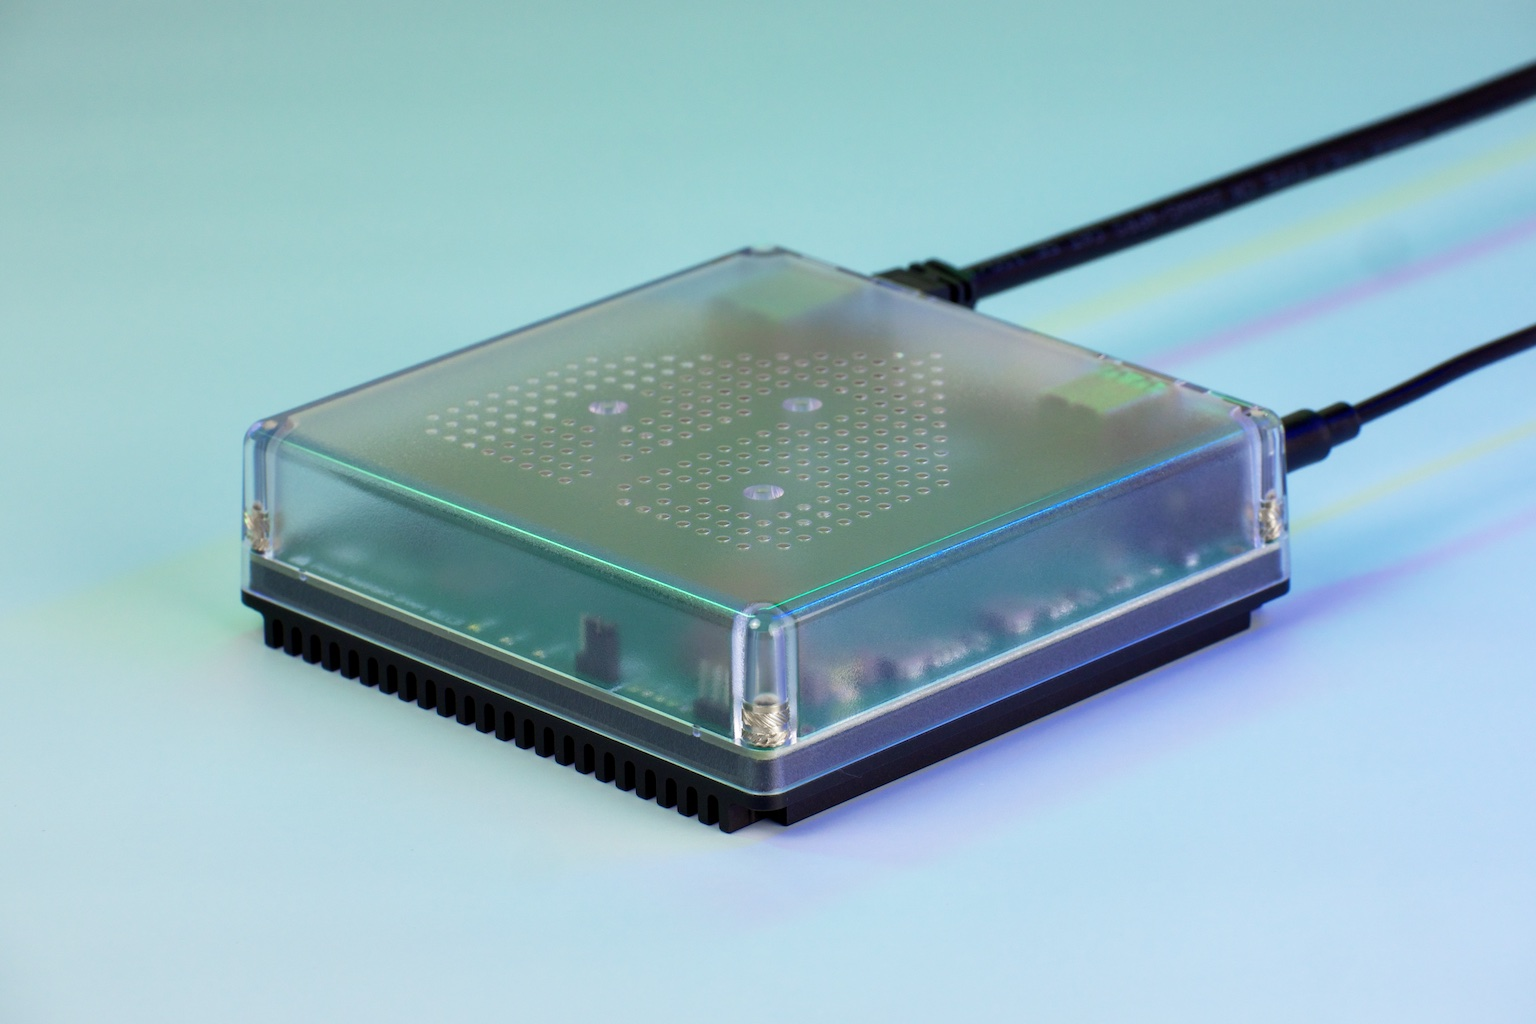
\includegraphics[width=.975\linewidth]{img/ha-green-photo-front.jpg}
        \caption{front of HAG \cite{HomeAssistant_HAG}}
    \end{subfigure}%
    \begin{subfigure}{.5\textwidth}
        \raggedleft
        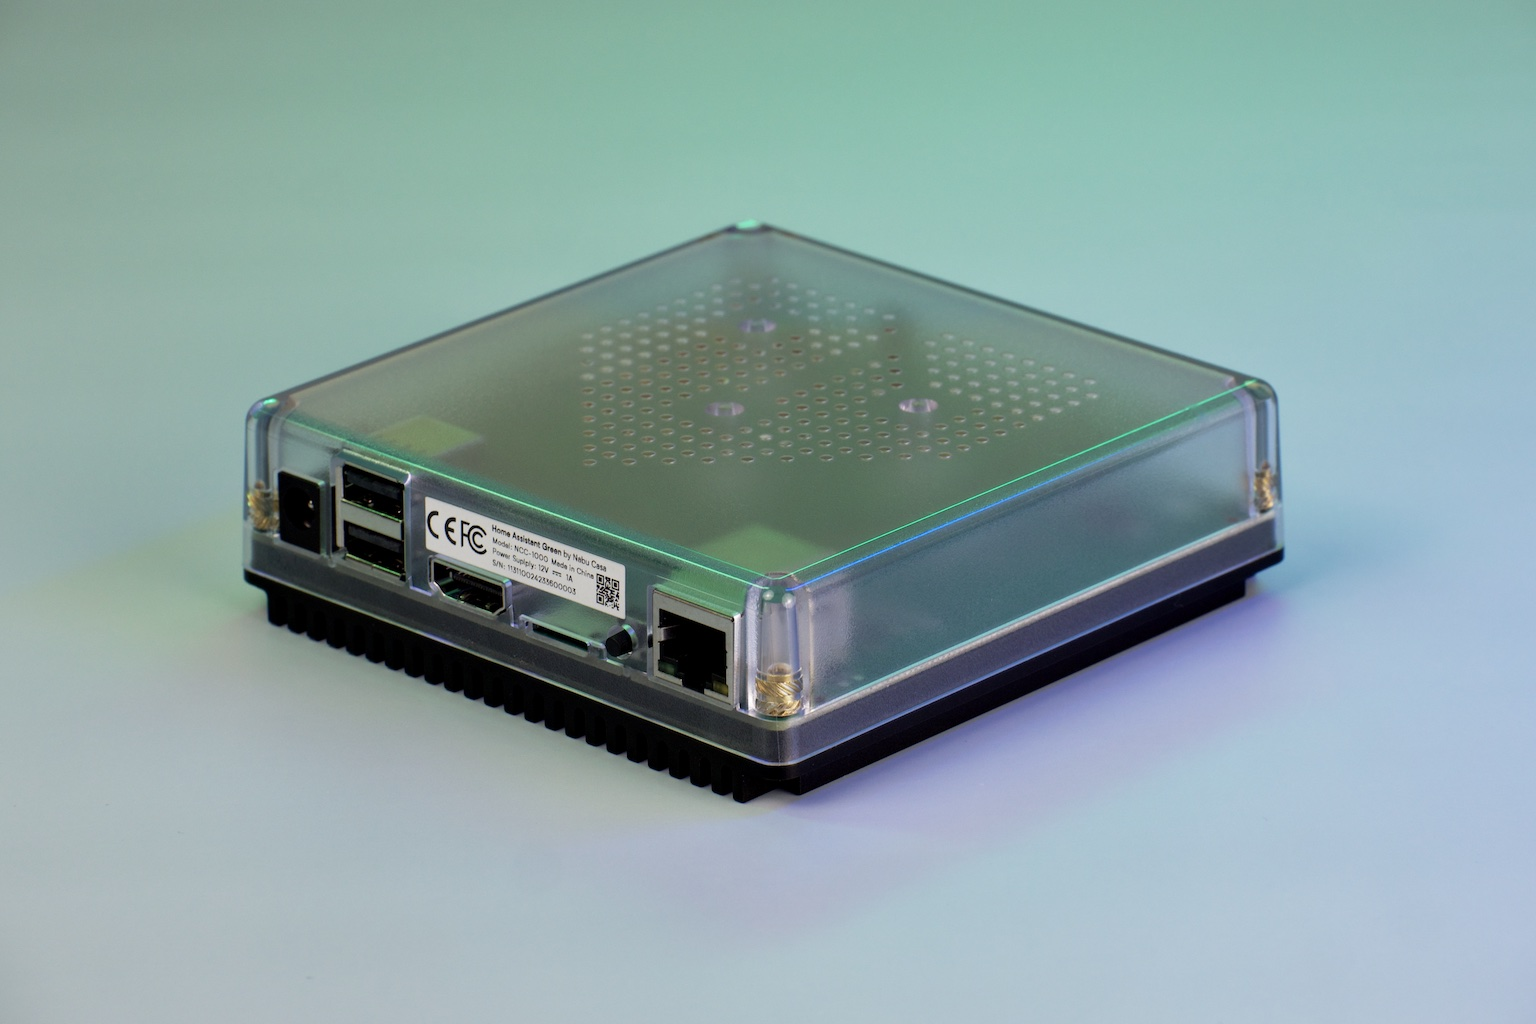
\includegraphics[width=.975\linewidth]{img/ha-green-photo-back.jpg}
        \caption{back of HAG \cite{HomeAssistant_HAG}}
    \end{subfigure}
    \caption{Home Assistant Green front and back side}
    \label{fig:HAG_front&back}
\end{figure}

\newpage

\subsubsection{Home Assistant on Raspberry Pi}
Installing Home Assistant on a Raspberry Pi is a DIY version of buying a Home Assistant Green. Assuming that the user wants to install the HA OS, the only additional tasks that they are required to perform is to flash the operating system to a micro SD card and assemble the Pi. The easiest way to flash the OS is to use the official \href{https://www.raspberrypi.com/software/}{Raspberry Pi Imager}\footnote{https://www.raspberrypi.com/software/} that supports Home Assistant as a pre-configured operating system \cite{HomeAssistant_Installation_Pi}. Apart from flashing the SD card, the installation is identical to HAG.

For the Pi itself Home Assistant recommends to either use an \href{https://www.raspberrypi.com/products/raspberry-pi-5/}{Raspberry Pi 5}\footnote{https://www.raspberrypi.com/products/raspberry-pi-5/} or \href{https://www.raspberrypi.com/products/raspberry-pi-4-model-b/}{Raspberry Pi 4}\footnote{https://www.raspberrypi.com/products/raspberry-pi-4-model-b/}, but for most cases even a \href{https://www.raspberrypi.com/products/raspberry-pi-3-model-b/}{Raspberry Pi 3 B}\footnote{https://www.raspberrypi.com/products/raspberry-pi-3-model-b/} should be fine \cite{HomeAssistant_Installation_Pi}, although the system could become slower once Home Assistant gets used more heavily.

\begin{figure}[H]
    \centering
    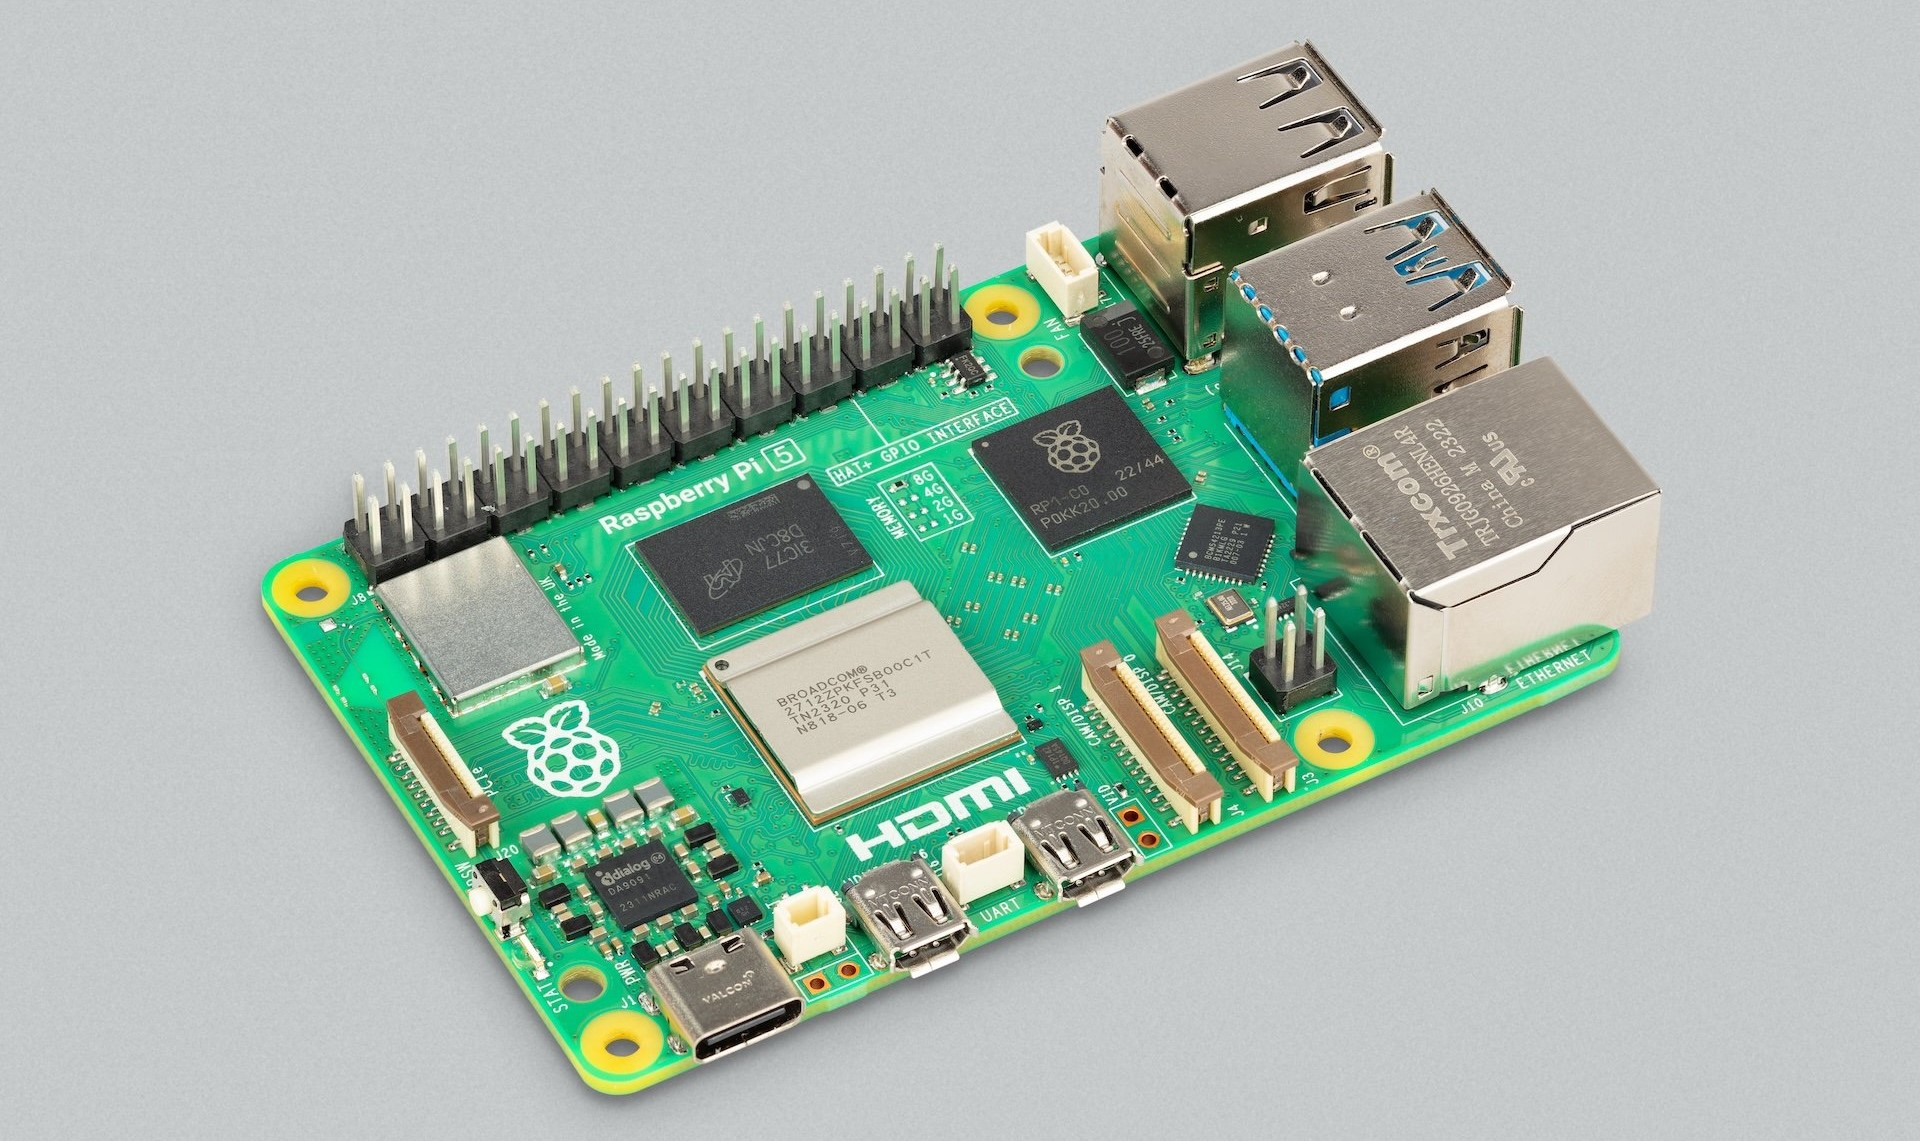
\includegraphics[width=.95\linewidth]{img/raspb-pi-5.jpg}
    \caption{Raspberry Pi 5 \cite{RaspberryPi_Doc_Pis}}
    \label{fig:HA-PI}
\end{figure}

\newpage

\subsubsection{Home Assistant Yellow}
The Home Assistant Yellow (HAY) is the advanced option of Home Assistant Green. It was designed to be an upgradable and extendable smart home hub that provides advanced features like a M.2 expansion slot and a \href{https://csa-iot.org/all-solutions/zigbee/}{Zigbee}\footnote{https://csa-iot.org/all-solutions/zigbee/}~\&~\href{https://www.threadgroup.org/}{Thread}\footnote{https://www.threadgroup.org/} multi-protocol radio, which are both wireless protocols for IoT-devices. The core of the HAY is a \href{https://www.raspberrypi.com/products/compute-module-4/}{Raspberr Pi Compute Module}\footnote{https://www.raspberrypi.com/products/compute-module-4/} that can be swapped out in the future to increase the compute power of the hub \cite{HomeAssistant_HAY}. The HAY is not as widely available as the HAG and is sold at a price roughly around €~150 \cite{mauser_HAY} (depending on the vendor and configuration).

The HAY can be bought in two flavours as either a preassembled device with Home Assistant already installed, or as a standalone kit without the Raspberry Pi Compute Module. However, the kit has the advantage that it is also available as a power-over-ethernet option. The preassembled device offers the same easy starting experience as the Home Assistant Green, where just a power and network cable must be plugged in. The kit requires the user to not only assemble the device, but also flash the operating system similarly to the Raspberry Pi \cite{HomeAssistant_HAY}.

\begin{figure}[H]
    \centering
    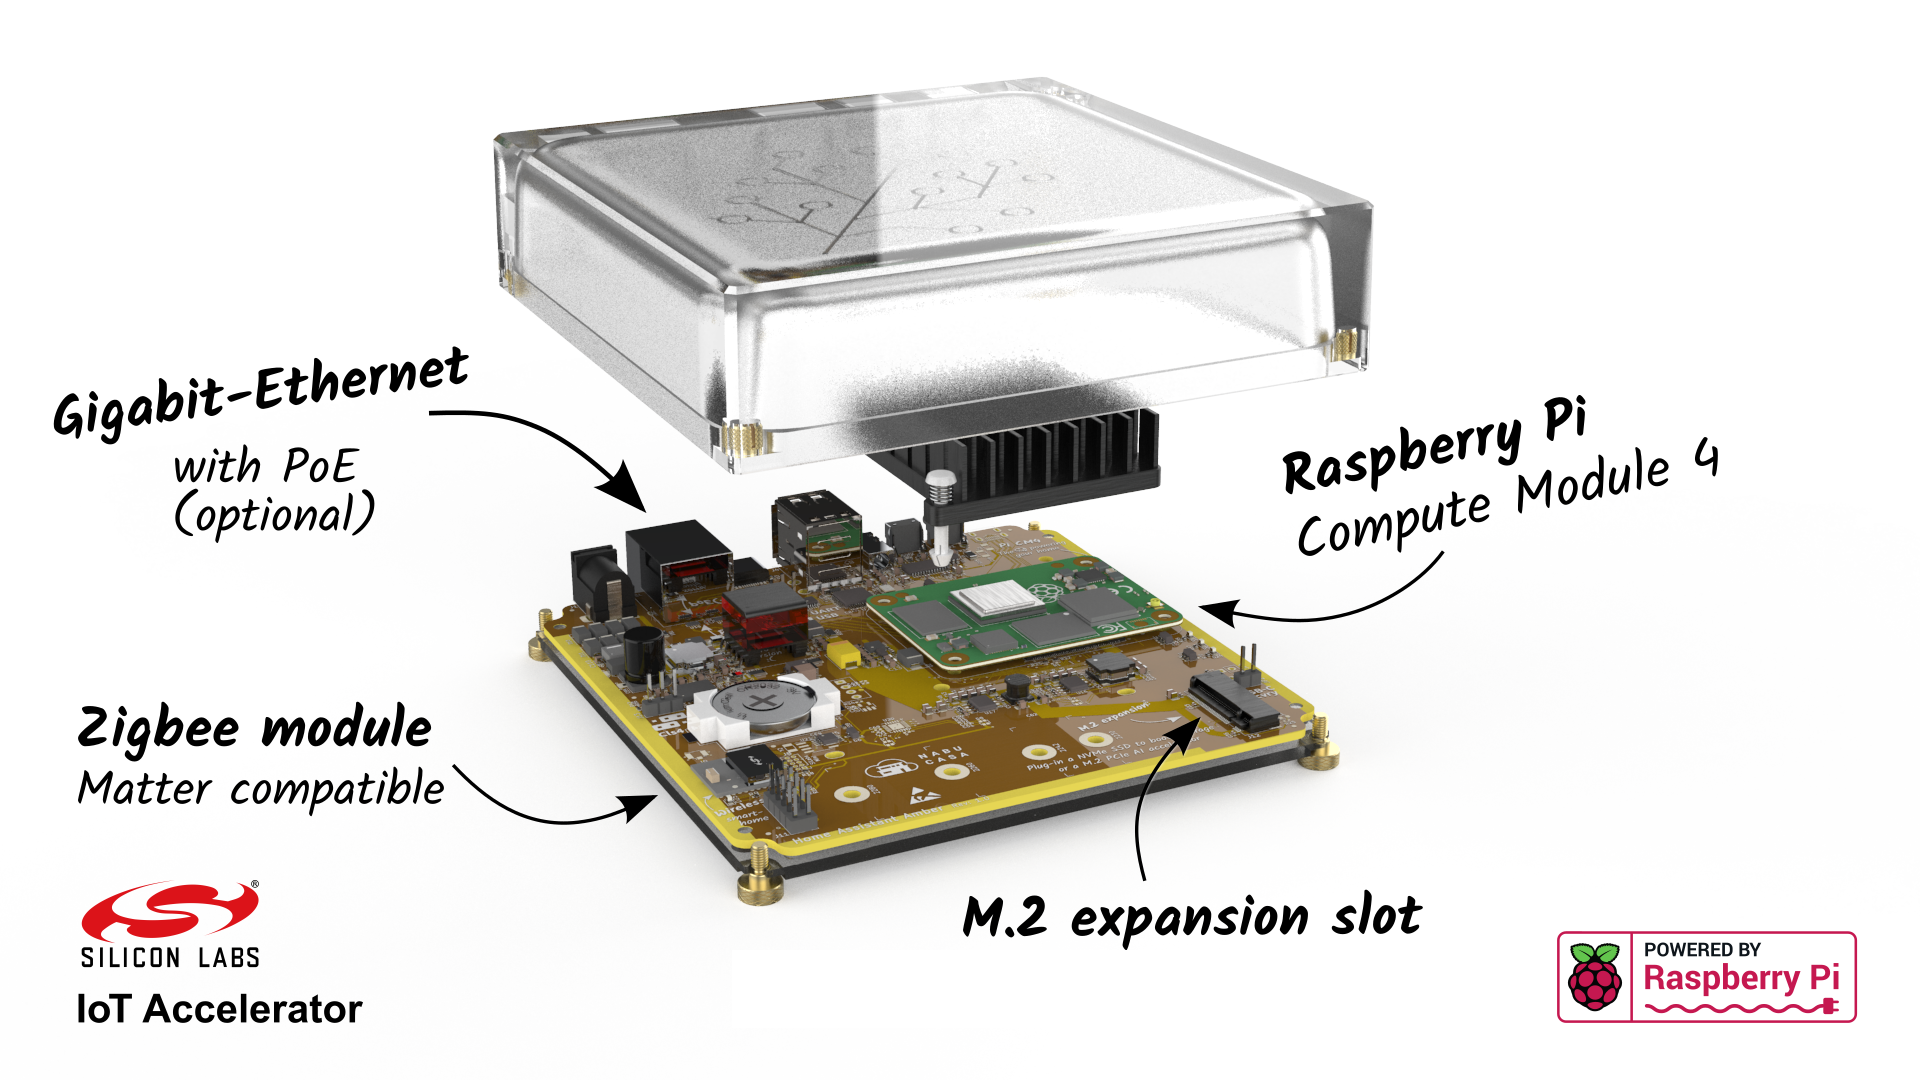
\includegraphics[width=.95\linewidth]{img/ha-yellow-labeled.png}
    \caption{Home Assistant Yellow \cite{HomeAssistant_HAY}}
    \label{fig:HA-Yellow-labeled}
\end{figure}

\subsection{Concepts and Terminology}
Home Assistant generally uses a similar terminology to other smart home platforms, but there is more depth to commonly used concepts. For example, most smart home platforms just know \textit{devices} themselves, but in HA devices consist of multiple \textit{entities}. To establish an understanding of those concepts in HA, the following paragraphs provide a brief overview of the most important ones.

\paragraph{Integrations}
To bring devices into HA, software modules called \textit{integrations} are required that allow HA to connect to external hardware or software controllers. This could be a bridge (e.g. Philips Hue Bridge) or devices themselves (e.g. Shelly relays). Integrations enable third party devices to be controlled by Home Assistant \cite{HomeAssistant_Docs_Concepts}. They provide connections to devices with proprietary vendor-specific protocols, connectivity standards such as \href{https://csa-iot.org/all-solutions/matter/}{Matter}\footnote{https://csa-iot.org/all-solutions/matter/} or Zigbee, but also to cloud services.

\begin{figure}[H]
    \centering
    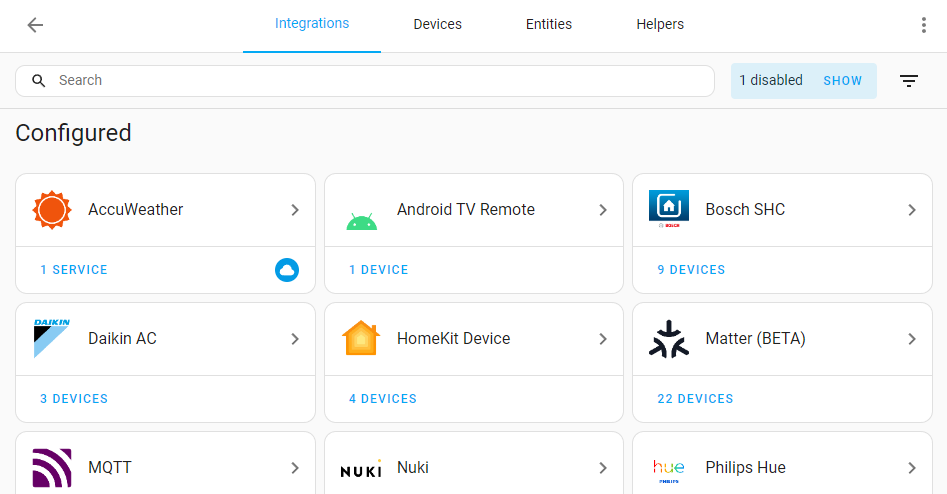
\includegraphics[width=.95\linewidth]{img/ha-integrations-configured.png}
    \caption{Example of configured integrations in Home Assistant}
    \label{fig:HA-Integrations-Configured}
\end{figure}

\paragraph{Entities}
Capabilities of devices are encapsulated in \textit{entities} that each house or control a single physical property or functionality of a device. The stored information is exposed as the entity's state. A state can only be one value at a time, but further information related to the current state can be stored in the entities attributes \cite{HomeAssistant_Docs_Concepts}. Moreover, a entity is uniquely distinguishable by its \textit{entity ID} and is a member of a entity domain. For example, a light facet (a device) would have an entity of the "light" domain with either a state of "on" or "off" that controls the output of a single light source. The brightness and color values of this light could then be stored as attributes that update as the state changes. If the facet has multiple independent light sources, they each would be exposed as their own entities.

\paragraph{Devices}
One \textit{device} typically consists of multiple entities and is associated with an integration. Devices can therefore be viewed as a logical grouping of entities that represents a physical or logical unit of some type but most commonly refer to physical devices/objects \cite{HomeAssistant_Docs_Concepts}. For example, a motion sensor often monitors additional attributes of a rooms like brightness or humidity, but also has internal attributes like the battery state or device temperature. Each of these sensors would be exposed as a single entity with its own state, but all are grouped \textit{in} the device and shown as one physical object.

\begin{figure}[H]
    \centering
    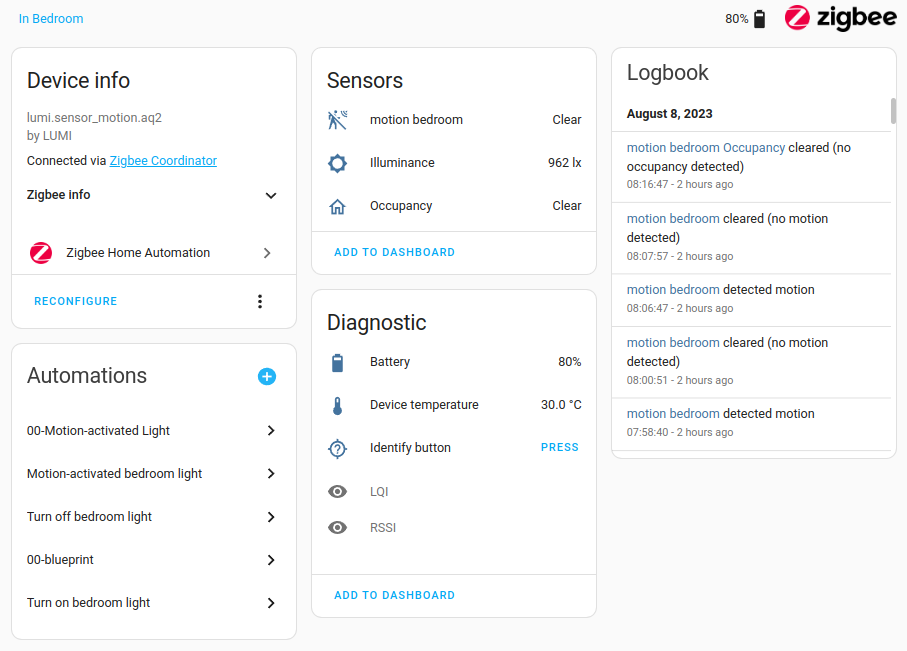
\includegraphics[width=.95\linewidth]{img/ha-device-example.png}
    \caption{Example of a motion sensor device shown in Home Assistant (Modified from \cite{HomeAssistant_Docs_Concepts})}
    \label{fig:HA-Device-Motion-Sensor}
\end{figure}

\paragraph{Areas}
\textit{Areas} are another level of logical grouping for devices and behave similar to \textit{rooms} in other smart home platforms. They are meant to represent physical rooms of the user's home and can also be assigned to a floor \cite{HomeAssistant_Docs_Concepts}.

\paragraph{Service calls}
\textit{Service calls} roughly compare to an API interface for a smart home. A service performs one specific action like turning on a light and is registered to a domain of entities that it can be called on. Services are a powerful tool for automations and scripts, but can also be used for controlling many devices at once. A service can target specific entities, devices, areas and labels (another user-defined level of grouping) \cite{HomeAssistant_Docs_Services}. While services are not meant to be manually called on a daily basis, they are vital for automating tasks. See Figure \ref{fig:HA-Service-Calls} for an usage example.

\begin{figure}[H]
    \centering
    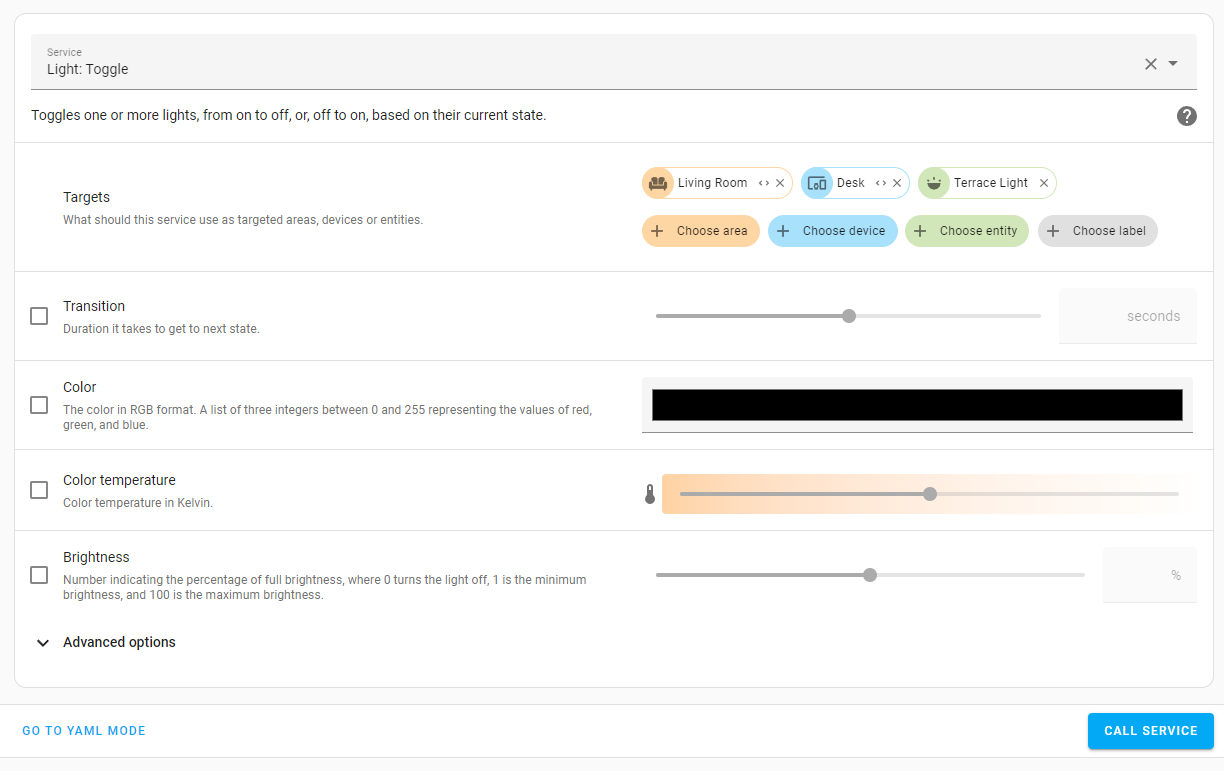
\includegraphics[width=.95\linewidth]{img/ha-service-calls.png}
    \caption{Example of a service call in Home Assistant}
    \label{fig:HA-Service-Calls}
\end{figure}

\paragraph{Automations}
At the surface, \textit{automations} in HA work and behave identical to other smart home platforms. However, they offer unparalleled possibilities and flexibility for automating even the most complex tasks by leveraging logical operators, loops, blocks for waiting on additional triggers, variables and so much more. Automations are assessed in further detail in section \ref{sec:ha-automations}.

\paragraph{Scripts}
A \textit{script} is similar to an automation, but is not run automatically by a trigger. Instead it is manually run by the user or by another automation. Scripts can also be exposed on the dashboard of HA \cite{HomeAssistant_Docs_Concepts}. 

\paragraph{Scenes}
\textit{Scenes} are a common concept in smart home and in HA they work identically to other platforms. They set an environment to a predefined state, without having to control every device individually \cite{HomeAssistant_Docs_Concepts}. 

\paragraph{Add-ons}
If HA was installed using one of the methods described in section \ref{sec:ha-installation}, the system supports the installation of \textit{add-ons}, which are containerised third-party applications that offer additional functionality. In contrast to integrations that connect HA to other apps/bridges, add-ons host new applications \cite{HomeAssistant_Docs_Concepts}. More about add-ons in section \ref{sec:ha-addons}.

\subsection{Device Support}
One of the main strengths of Home Assistants is the vast support they receive from the open source community. This particularly shows in the number of integrations that are available for HA. In total, the \href{https://www.home-assistant.io/integrations}{official integration store}\footnote{https://www.home-assistant.io/integrations} offers \textbf{2831 unique integrations} \cite{HomeAssistant_Integrations} (as of July 8, 2024).

However, this is only the set of \textit{officially} supported integration. Home Assistant can be extended by anyone at any time and one of this extensions is \href{https://hacs.xyz/}{HACS}\footnote{https://hacs.xyz/} (Home Assistant Community Store) \cite{HACS_Homepage}, which houses many further integrations. Therefore, chances are that if a device is supported by any smart home platform, it would be Home Assistant.

\newpage

\subsection{Out-of-home Control}
\label{sec:ha-remote-access}
Since everything in Home Assistant runs locally, remote access is more difficult than on other smart home platforms. In general, there are three approaches for setting up out-of-home control \cite{HomeAssistant_Remote_Access}:

\begin{itemize}
    \item \textbf{Home Assistant Cloud} - the HA subscription service that provides, amongst other things, end-to-end encryption for remote access
    \item \textbf{VPN} - secure remote connection into the own home network
    \item \textbf{Port forwarding} - exposing Home Assistant to the internet
\end{itemize}

Although all of these options are possible to deploy securely, port forwarding requires some technical proficiency and is not suitable for every installation. Therefore, it is not recommended for the average user. To give some basic understanding of how the three options are deployed in Home Assistant, the following paragraphs will briefly touch on the matter.

\paragraph{Home Assistant Cloud}
This is the easiest option for remote access, but requires a subscription at Nabu Casa. Home Assistant Cloud provides the user with a unique remote URL and a certificate to encrypt the traffic between the user's devices and the HA instance. The subscription itself costs €~7.50 per month, or €~75 annually \cite{NabuCasa_Pricing} and directly funds the development of Home Assistant. Besides creating an account and logging in, this option does not require further setup \cite{HomeAssistant_Remote_Access}.

\paragraph{VPN}
A Virtual Private Network (VPN) enables the user to remotely access the resources on their home network as long as they are connected via the VPN service. Home Assistant offers a few options for hosting a VPN server by installing an application via the add-on store. HA features two VPN services on their documentation page that are easy to setup: \href{https://tailscale.com/}{Tailscale}\footnote{https://tailscale.com/} and \href{https://www.zerotier.com/}{ZeroTier One}\footnote{https://www.zerotier.com/} \cite{HomeAssistant_Remote_Access}. Both of their free-tier services are sufficient for most use cases.

\paragraph{Port forwarding}
Setting up port forwarding means exposing the Home Assistant instance publicly. Therefore, in no circumstances should this be done without setting up proper end-to-end encryption, which requires a \textit{public domain} and a \textit{certificate}. Since some Internet Service Providers only offer dynamic IP addresses, this is easiest done by using a \textit{Dynamic DNS service} \cite{HomeAssistant_Remote_Access} like \href{https://www.duckdns.org/}{DuckDNS}\footnote{https://www.duckdns.org/} and a \textit{certificate service} like \href{https://letsencrypt.org/}{Let's Encrypt}\footnote{https://letsencrypt.org/}, which both are completely free of charge. For setting this up with Home Assistant the user can install the \href{https://github.com/home-assistant/addons/blob/master/duckdns/DOCS.md}{DuckDNS add-on}\footnote{https://github.com/home-assistant/addons/blob/master/duckdns/DOCS.md} from the add-on store and follow the instructions from their documentation. In essence, after installation, the user is required to register an account at DuckDNS, select a free domain name, copy an API token \& domain to the configuration of the add-on, and accept the Let's Encrypt terms of service. Everything else, including renewal of the certificate, is done by the application \cite{HomeAssistant_DuckDNS_github}. After exposing a port on the router the HA instance should be remotely accessible. However, access is of course still protected by user credentials and two-factor authentication. 

\subsection{Dashboards}
Home Assistants' approach on dashboards is somewhat different to most smart home platforms. While e.g. Apple Home exposes all of the users devices on the dashboard as soon as they are added to the smart home system, HA wants the user to \textit{create and layout} their dashboard according to their personal liking and handle device management on a separate device panel in the settings. Moreover, Home Assistant allows the user to create as many dashboards as they want.

This approach offers the advantage that dashboards can be more refined, personalised, and specialised than in most smart home systems, but also means that devices have to be explicitly added to the dashboard, which can be time consuming at first. 

Home Assistant provides a live \href{https://demo.home-assistant.io/}{interactive dashboard demo}\footnote{https://demo.home-assistant.io/} (also visible in Figure \ref{fig:HA-Dashboard-Demo}) so that everyone can form their personal opinion about this system without requiring HA to be installed in advance. On that website, one can also view different dashboard designs that were made by the community.

A further advantage of dashboards in HA is that everything can be customised by either the UI or CSS styling. Alternatively, users can also download or create custom themes \cite{HomeAssistant_Frontend} to style their whole interface.

\begin{figure}[H]
    \centering
    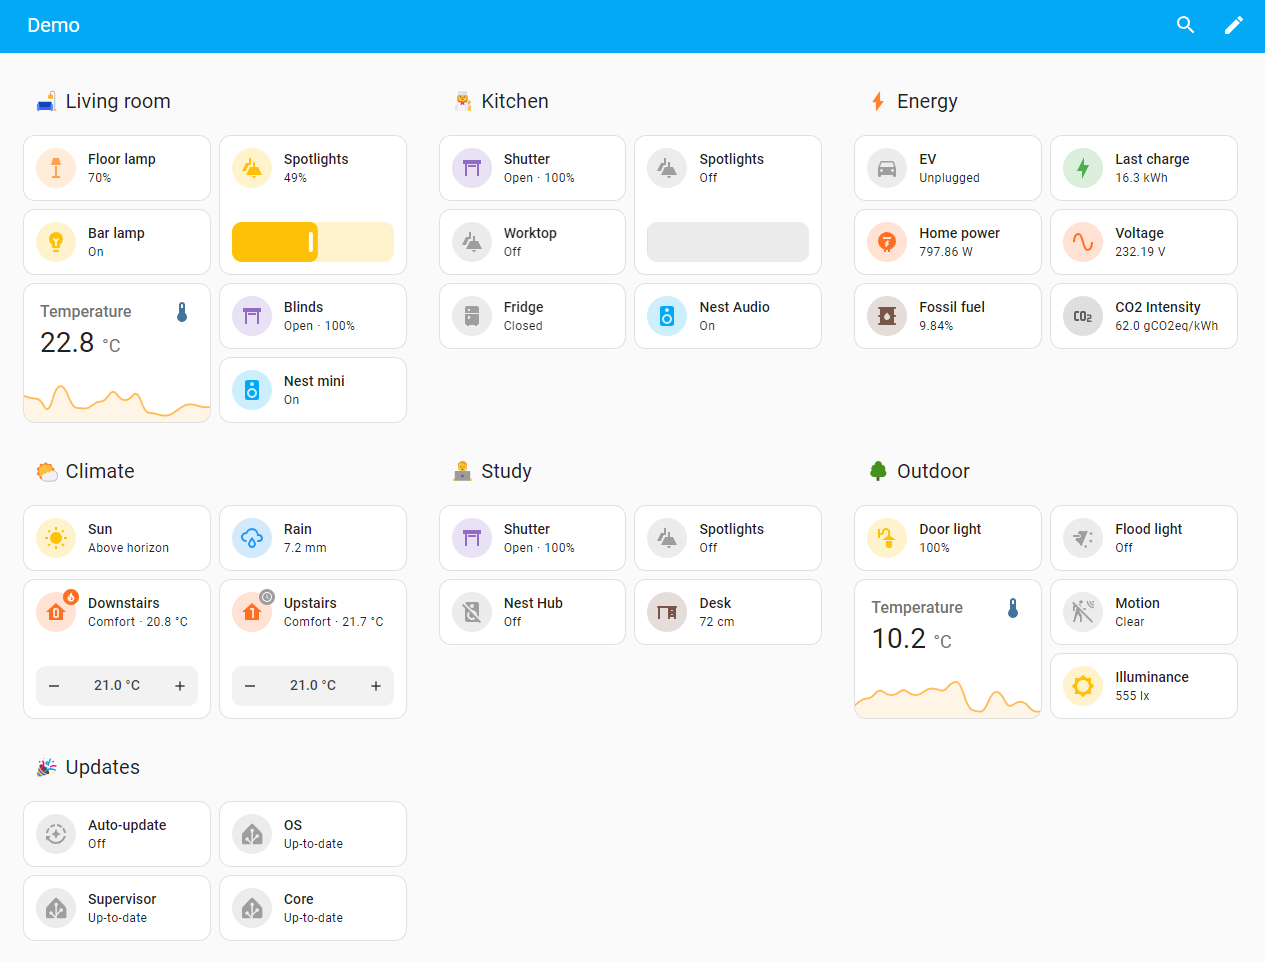
\includegraphics[width=.95\linewidth]{img/ha-dashboard-demo.png}
    \caption{Interactive HA dashboard demo \cite{HomeAssistant_Dashboard_Demo}}
    \label{fig:HA-Dashboard-Demo}
\end{figure}

The dashboard can be adapted by entering the edit mode (pencil icon at the top right corner). In this mode cards can be rearranged by drag and drop, and created by clicking on the marked empty spaces in their section. The edit UI is shown in Figure \ref{fig:HA-Dashboard-Demo-Editing}.

\begin{figure}[H]
    \centering
    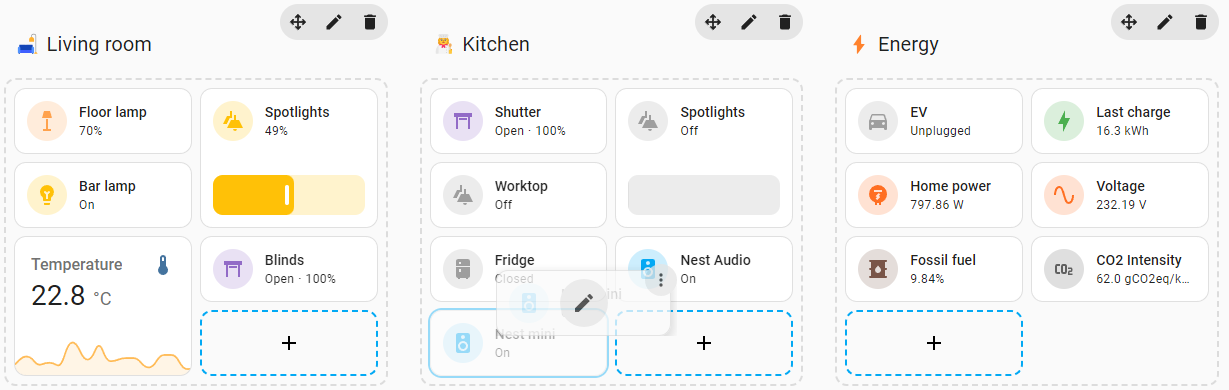
\includegraphics[width=.95\linewidth]{img/ha-dashboard-demo-editing.png}
    \caption{Interactive HA dashboard demo - Editing of a dashboard \cite{HomeAssistant_Dashboard_Demo}}
    \label{fig:HA-Dashboard-Demo-Editing}
\end{figure}

Cards can also be configured to the users liking by adding additional control options (called \textit{Features} in the UI), changing the default tap actions when clicking either the icon or the card background and changing the whole size of the card in the grid. Furthermore, they can be shown conditionally when, e.g. an entity has a state or on a per-user basis.

\begin{figure}[H]
    \centering
    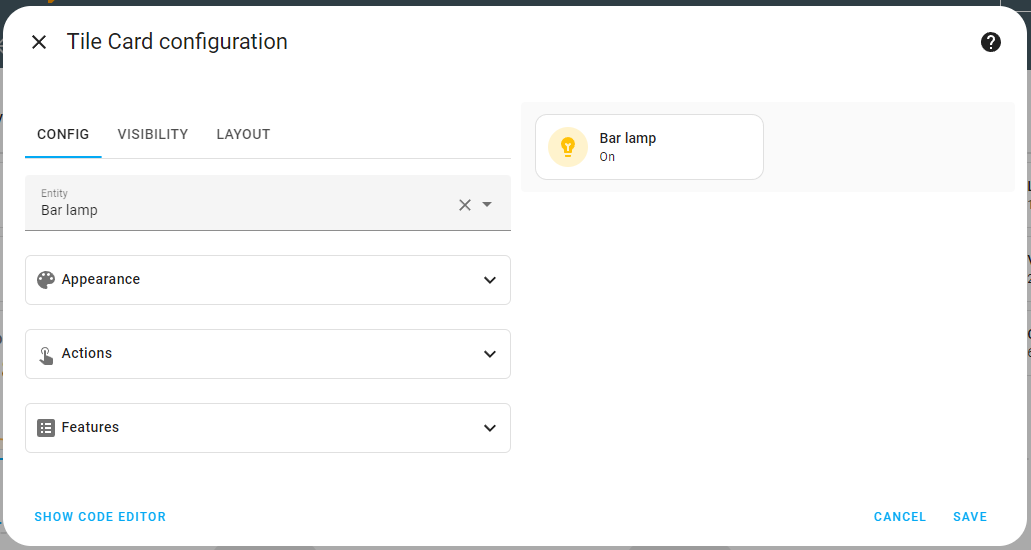
\includegraphics[width=.95\linewidth]{img/ha-dashboard-demo-editing-card.png}
    \caption{Interactive HA dashboard demo - Editing of a card on the dashboard \cite{HomeAssistant_Dashboard_Demo}}
    \label{fig:HA-Dashboard-Demo-Editing-Card}
\end{figure}

In essence, everything on the HA dashboards can be configured and extended, especially when considering adding custom cards from the aforementioned Home Assistant Community Store.

\subsection{Automations}
\label{sec:ha-automations}

In their basic form, automations are made up of three components \cite{HomeAssistant_Docs_Services}:

\begin{enumerate}
    \item \textbf{Triggers} - the event that starts the automation
    \item \textbf{Conditions} - an optional test that has to pass before actions run
    \item \textbf{Actions} - the tasks the automation should perform
\end{enumerate}

Automations can be triggered by any event in Home Assistant. This includes state changes of devices/entities, on a specific time or time pattern, location events, scanning NFC Tags or even by triggering webhooks and many more. The conditions are similar to triggers, but relate to the current state, rather than a state change of some entity.

Actions are almost limitless in their capabilities for automation. In addition to controlling devices and calling services, actions include various building blocks that represent loops and logic known from traditional programming like \textit{If-then}, \textit{Repeat} (while-loop), \textit{Variables}, \textit{Choose} (switch statement) and \textit{delays}. Furthermore, there are complex building blocks for waiting on additional triggers or checking for conditions further down in the action sequence, and for running actions in sequence or in parallel. 

An easy way to get started with setting up automations is to use \href{https://www.home-assistant.io/docs/automation/using_blueprints/}{community made blueprints}\footnote{https://www.home-assistant.io/docs/automation/using\_blueprints/} which can be imported into HA with a single button from the forums. Later, these blueprints can be configured and edited by the user \cite{HomeAssistant_Automation_Blueprints}.

\subsection{History}
Since devices in a smart home generate a lot of data, exploring historic data can be valuable. The \textit{History} panel in Home Assistant allows the user to view the state changes of an entity over time. By default, HA stores the full historic data for ten days (can be modified). After that period, long term statistical data is generated which averages one data point per hour~\cite{HomeAssistant_History}. However, these long term statistics are only generated for entities with continuous variables, like temperature, as storing and condensing discrete states, such as switch statuses, is generally less useful and more challenging.

\begin{figure}[H]
    \centering
    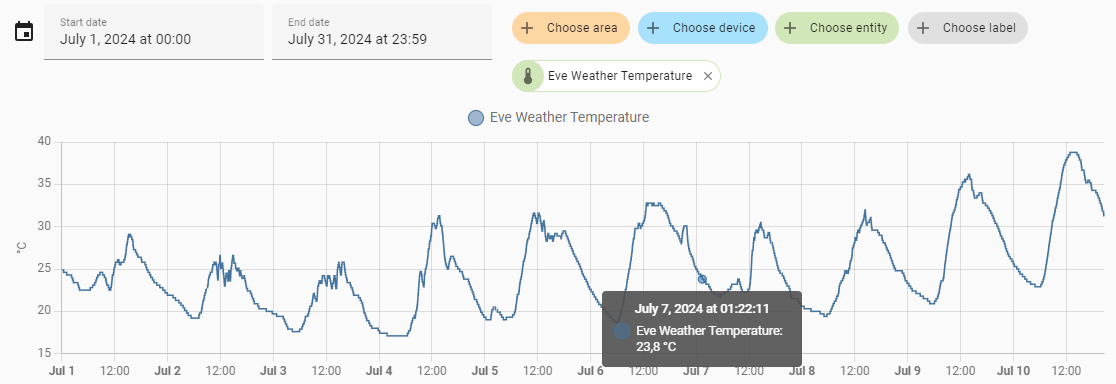
\includegraphics[width=.95\linewidth]{img/ha-history.png}
    \caption{Example of a temperature sensor in the History panel of Home Assistant}
    \label{fig:HA-History}
\end{figure}

\subsection{Voice Assistant}
\label{sec:ha-voice-assistant}
Home Assistant offers the possibility to either integrate a third-party voice assistant into HA, or use their own implementation called \textit{Assist}.

Either Google Assistant or Amazon Alexa are supported as third-party voice assistants \cite{HomeAssistant_VoiceControl}. They can be integrated manually (DIY option) \cite{HomeAssistant_GoogleAssistant}\cite{HomeAssistant_AmazonAlexa} or by using Home Assistant Cloud \cite{NabuCasa_Startpage}, but the later is the recommended simpler solution.

\textit{Assist} is the voice assistant interface developed by Home Assistant, but it is rather different to setup than traditional voice assistants. Assist is composed of three components that form the \textbf{Assist pipeline}:

\begin{itemize}
    \item \textbf{Conversation agent} - the brain of the voice assistant that processes incoming text commands
    \item \textbf{Speech-to-text} - engine for converting voice to text
    \item \textbf{Text-to-speech} - engine for converting text to voice
\end{itemize}

Each of these components can be configured or swapped out by the user, and only the conversation agent comes pre-installed with Home Assistant~\cite{HomeAssistant_VoiceControl}. However, without the other two components Assist can only process incoming text commands and answer with text output.

HA provides two options to solve this. Either subscribe to Home Assistant Cloud and use the compute power of their cloud servers \cite{HomeAssistant_Assist_Cloud}, or \textbf{host them locally} \cite{HomeAssistant_Assist_Local}. Home Assistant provides users the possibility to have full agency over their voice assistant, a feature that no traditional smart home platform offers.

For setting this up locally, the user must install and configure \href{https://github.com/SYSTRAN/faster-whisper}{faster-whisper}\footnote{https://github.com/SYSTRAN/faster-whisper} for the speech-to-text and \href{https://github.com/rhasspy/piper}{Piper}\footnote{https://github.com/rhasspy/piper} for the text-to-speech component \cite{HomeAssistant_Assist_Local}. Both are available in the add-on store inside of Home Assistant. Afterwards, the Assist pipeline can be re-configured to use the two components. Although this configuration can even be hosted on a Raspberry Pi, more powerful hardware is advised for achieving comfortable response times. For example on a Raspberry Pi 4 faster-whisper takes eight seconds to process incoming voice commands. On a Intel NUC, this can be done in under one second \cite{HomeAssistant_Assist_Local}.

Counterparts to stationary devices similarly to e.g. an Amazon Echo can also be installed for using the Assist as a traditional voice assistant. These voice satellites can be build with, amongst others, an ESP-based device \cite{HomeAssistant_VoiceControl} like the \href{https://www.home-assistant.io/voice_control/s3_box_voice_assistant/}{ESP-S3-BOX-3}\footnote{https://www.home-assistant.io/voice\_control/s3\_box\_voice\_assistant/} \cite{HomeAssistant_Assist_S3Box}, but even tiny boards like the \href{https://www.home-assistant.io/voice_control/thirteen-usd-voice-remote/}{ATOM~Echo}\footnote{https://www.home-assistant.io/voice\_control/thirteen-usd-voice-remote/} that is available for as little as \$~13 work with Assist \cite{HomeAssistant_Assist_AtomEcho}.

For these voice satellites Home Assistant supports wake-word detection for triggering Assist. Depending on the computing power of the device this can either be done by the HA server with the \href{https://github.com/dscripka/openWakeWord}{openWakeWord}\footnote{https://github.com/dscripka/openWakeWord} add-on, or on-device with \href{https://github.com/kahrendt/microWakeWord}{microWakeWord}\footnote{https://github.com/kahrendt/microWakeWord} \cite{HomeAssistant_WakeWord}. Furthermore, the model can be trained by the user to use custom wake-words \cite{HomeAssistant_CustomWakeWord}.

\subsection{Advanced Features: Beyond traditional Smart Home}

Home Assistant is built by the open source community, which is infamous for creating customisable and open software. On the past few pages, many different features were described, but HA has so much more to offer. Especially for users that want to deeper engage with their smart home. In the following few paragraphs, some of those advances topics will be briefly touched on.

\paragraph{Add-ons}
\label{sec:ha-addons}
Various add-ons such as Tailscale, DuckDNS, openWakeWord, and HACS were already mentioned previously and all show what additional capabilities third-party applications can add to Home Assistant. The add-on store enables these to be up and running in seconds, and they often do not require complex configuration. Further interesting add-ons to play with are, for example \href{https://grafana.com/}{Grafana}\footnote{https://grafana.com/}, which enables advanced data visualisation of the locally stored sensor data, or \href{https://grocy.info/}{Grocy} that is a self-hosted grocery and household management solution similar to an enterprise resource program. All of these are open source software that can be used together with HA, which in itself is a major advantage of using Home Assistant as a smart home platform.

\newpage

\paragraph{Data Science}
A smart home generates large amounts of data, which can be explored using data science in Home Assistant. For example, \href{https://github.com/hassio-addons/addon-jupyterlab}{JupyterLab}\footnote{https://github.com/hassio-addons/addon-jupyterlab} can be installed as an add-on in HA, enabling jupyter notebooks to access the HA database. Users interested in data science can follow the introduction and quick-start guide at the \href{https://data.home-assistant.io/docs/quick-start}{Home Assistant Data Science Portal}\footnote{https://data.home-assistant.io/docs/quick-start} to learn how to experiment with their own smart home data.

\paragraph{ESPHome}
The creators of Home Assistant also developed \href{https://esphome.io/index.html}{ESPHome}\footnote{https://esphome.io/index.html}, a system to control microcontrollers by writing simple configuration files. Furthermore, the devices integrate seamlessly into Home Assistant. This project enables DIY enthusiasts to control various appliances with e.g. ESP32 boards, expose them in HA, and update them easily \cite{ESPHome_Startpage}. For users interested in DIY projects, Home Assistant is a viable tool to integrate these projects into their smart home. An example of this is shown in figure \ref{fig:ESPHome_Poolcontroler}, where an ESP32-POE board is exposed in Home Assistant using the ESPHome project.

\begin{figure}[H]
    \centering
    \begin{subfigure}{.5\textwidth}
        \raggedright
        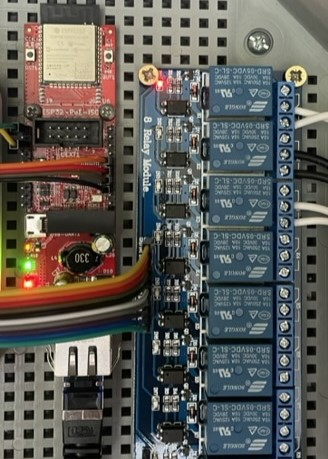
\includegraphics[width=.975\linewidth]{img/pool-controler.JPEG}
        \caption{ESP32-POE with relay board}
    \end{subfigure}%
    \begin{subfigure}{.5\textwidth}
        \raggedleft
        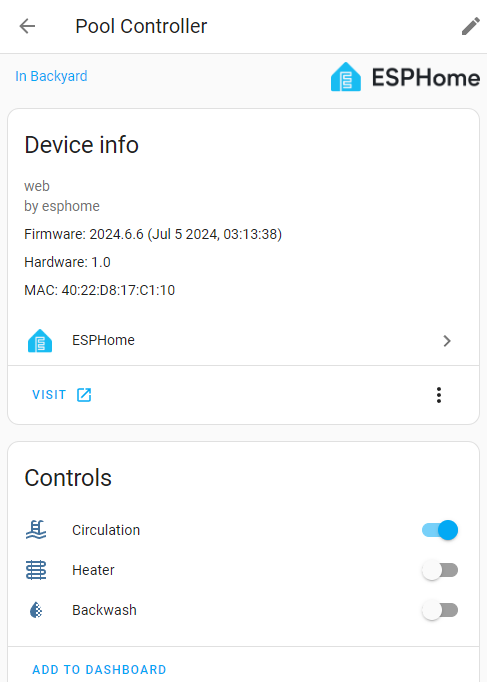
\includegraphics[width=.975\linewidth]{img/ha-esphome-pool-controler.png}
        \caption{ESPHome device exposed in HA}
    \end{subfigure}
    \caption{DIY pool controller running ESPHome}
    \label{fig:ESPHome_Poolcontroler}
\end{figure}

\newpage

%% Section 6 - SHP Comparison

\section{Comparison of Smart Home Platforms}

The aim of this chapter is to examine whether Home Assistant, as a locally hosted service, delivers a comparable set of capabilities in relation to traditional smart home platforms. For this the platforms were tested in an experiment and compared using a utility analysis.
The traditional smart home platforms tested in this comparison are Apple Home, Google Home, Samsung Smart Things and Amazon Alexa. Capabilities were evaluated by comparing the available \textbf{control options}, the offered \textbf{feature set}, the potential for configuring powerful \textbf{automations} and the abilities of the \textbf{voice assistant }associated with the respective smart home platform.
Control options and Features represent \textit{active tools} for users to interact with their smart home (e.g. controlling, monitoring, or gathering information), while Automations and Voice Assistant represent \textit{passive tools}, where the smart home executes actions on behalf of the user.
Although this framework does not cover all dimensions of smart home technology, such as supported protocols, reliability or system cost, its aim is to cover a basic smart home usage scenario. The mentioned attributes were furthermore deliberately ignored for this comparison, since they are heavily influenced by the protocols in use as shown in \cite{SHS-Overview&ComparativeAnalysis-8718722}.

All smart home platforms were tested with at the time of writing (24th of June 2024) officially supported (not deprecated) devices with the latest firmware installed. Except of the device used for Amazon Alexa, all devices are still sold by their respective companies and therefore could be newly deployed by a user who starts with smart home today.

\subsection{Evaluation Criteria}

The comparison is split in the aforementioned dimensions, which criteria are further specified in

\begin{itemize}
    \item Table \ref{tab:spec_control}: \nameref{tab:spec_control}
    \item Table \ref{tab:spec_features}: \nameref{tab:spec_features}
    \item Table \ref{tab:spec_automations}: \nameref{tab:spec_automations}
    \item Table \ref{tab:spec_voiceassistant}: \nameref{tab:spec_voiceassistant}
\end{itemize}

\noindent
Additional insight on the distinct smart home platforms can be found in section \ref{sec:obs_evaluation}.

\begin{table}[H]
    \centering
    \caption{Specification for Comparison of Control Options}
    \label{tab:spec_control}
    \begin{tabular}{ >{\raggedright} p{0.3\linewidth} p{0.65\linewidth} }
        \toprule
        \multicolumn{2}{ l }{\textbf{Control Options}} \\
        \midrule
        \textbf{Criteria} & \textbf{Requirement} \\
        \midrule
        Smartphone App & Offer a dedicated smartphone app \\ \addlinespace
        Cross-Platform Apps & Apps are available for iOS and Android phones \\ \addlinespace
        Web Interface & Smart home can be controlled via a web browser \\ \addlinespace
        Voice Assistant & Platform offers its own distinct voice assistant \\ \addlinespace
        Offline-Control & The interface can be controlled locally and therefore without an active internet connection \\ \addlinespace
        Out-of-Home & The interface is available while the user is outside their residential network \\ 
        \bottomrule
    \end{tabular}
\end{table}

\begin{table}[H]
    \centering
    \caption{Specification for Comparison of Features}
    \label{tab:spec_features}
    \begin{tabular}{ >{\raggedright} p{0.3\linewidth} p{0.65\linewidth} }
        \toprule
        \multicolumn{2}{ l }{\textbf{Features}} \\
        \midrule
        \textbf{Criteria} & \textbf{Requirement} \\
        \midrule
        Scenes & Change the state of multiple devices of different device-families simultaneously \\ \addlinespace
        Automations & Perform event-driven actions based on triggers \\ \addlinespace
        Combine Accessories & Group devices so that they can be controlled together \\ \addlinespace
        Combine Actions (Scripts/Flows) & Execute a sequence of actions with conditional logic \\ \addlinespace
        Locate Devices/People & Assist in finding phones or other tracked objects \\ \addlinespace
        Third-Party Extensions & Extend the base application with capabilities from third parties \\ \addlinespace
        Device State History & Show a record of state changes of specific devices over time \\ \addlinespace
        Event Logs & Show a record of activities, actions, or changes within the system \\ \addlinespace
        Energy Monitoring & Measure, record, and visualise the energy usage of devices over time \\
        \bottomrule
    \end{tabular}
\end{table}

\begin{table}[H]
    \centering
    \caption{Specification for Comparison of Automations}
    \label{tab:spec_automations}
    \begin{tabular}{ >{\raggedright} p{0.3\linewidth} p{0.65\linewidth} }
        \toprule
        \multicolumn{2}{ l }{\textbf{Automations}} \\
        \midrule
        \textbf{Criteria} & \textbf{Requirement} \\
        \midrule
        Time based trigger & Turn on the garden lights at 8pm.\\ \addlinespace
        Location based trigger & Lock the door when the user leaves the house.\\ \addlinespace
        Send notifications based on events & Send a notification if the door gets opened after 10pm.\\ \addlinespace
        Simple Conditional Logic & Turn a light on if motion gets detected after 10pm.\\
        \bottomrule
    \end{tabular}
\end{table}

\begin{table}[H]
    \centering
    \caption{Specification for Comparison of Voice Assistants}
    \label{tab:spec_voiceassistant}
    \begin{tabular}{ >{\raggedright} p{0.3\linewidth} p{0.65\linewidth} }
        \toprule
        \multicolumn{2}{ l }{\textbf{Voice Assistants}} \\
        \midrule
        \textbf{Criteria} & \textbf{Requirement} \\
        \midrule
        Obtain external information & “How is the weather today?” – provide forecast \\ \addlinespace
        Perform actions & “Turn off the lights in this room.” – turn off lights \\ \addlinespace
        Set a reminder & “Remind me to go grocery shopping tomorrow 10am.” – add a reminder \\ \addlinespace
        Set a timer & “Set a timer for 10 minutes.” – sound an alarm in 10 minutes \\ \addlinespace
        Identify voice of household members & “Who am I?” – enable personal requests by distinguishing voices \\
        \bottomrule
    \end{tabular}
\end{table}

\newpage

\subsection{Insight into the compared Platforms} \label{sec:obs_evaluation}

This section will briefly describe the most relevant key-facts of each smart home platform and point out important information for the final comparison.

\subsubsection{Apple Home}
Apple Home (AH) has been tested using a Apple HomePod mini with the firmware 17.5 (21L569) and an iPhone 12 Pro with the latest operating system version iOS 17.5.1 installed.

\paragraph{Control Options}
AH exclusively offers apps for Apple devices and therefore excludes household members that use Android smartphones or Windows PCs. Its voice assistant is called \textit{Siri} which can execute some voice commands locally and communicates with iPhones on the same network to receive personal information, but depends on external servers for more complex tasks. Out-of-home control is available through Appels iCloud Service.

\paragraph{Features}
In terms of features HA mainly focuses on basic capabilities. Devices of the same type can be grouped to display as a single entity, for example, the individual lights of a chandelier, and scenes can be created to control multiple devices simultaneously. An event history is available, but this is limited to only include smart locks and garage doors. However, more complex features, such as viewing the state history of devices or energy monitoring, are currently missing.

\paragraph{Automations}
AH supports the most common event triggers for automations like people arriving/leaving a place, accessories changing their state (being controlled or sensors detecting something) and time-based events. The action flow that can be executed within an automation is limited to setting the state of devices. Logical operations like if-then, conditionally waiting on another event or for time to pass are not supported. The only exception are lights, which can be turned off again after a set amount of time.

\paragraph{Voice Assistant}
Although Siri is commonly perceived as a rather weak voice assistant, it satisfies all the criteria of this test.

\newpage
\subsubsection{Google Home}
Google Home (GH) has been tested using a Google Nest Mini with the firmware 2.57.375114.

\paragraph{Control Options}
GH is mainly focused on controlling smart home devices with their voice assistant \textit{Google Assistant}.
Out-of-home control is available through the Google Cloud. However, most smart home devices stop working once the hub loses its connection to the Internet. Presumably only devices that directly connect to the phone, such as some smart TVs, remain controllable. Google recently confirmed that they are working on implementing some form of local control \cite{Reddit_r/GoogleHome2023OfflineMode}.

\paragraph{Features}
Scenes are not directly integrated into the GH app. External applications can provide scenes to the Google Assistant API \cite{GoogleDeveloper2023ScenesGuide}, but it is not supported to create new scenes within the GH app. Third-party integrations are available with Google Cloud. Energy monitoring is only available for thermostats, but not for power plugs. This means that heat can be monitored, but electricity can not.

\paragraph{Automations}
GH distinguishes between \textit{Household Routines} and \textit{Personal Routines}, but for this smart home comparison only the household routines are relevant. Automation triggers can be voice commands, a specific time or an alarm on a smart speaker. Noteworthy about GHs automation is that they provide a web interface for configuring advanced routines.

\paragraph{Voice Assistant}
GH is heavily focused on using its voice assistant as the primary interaction interface and had no shortcomings in the comparison.

\newpage
\subsubsection{Samsung Smart Things}
Samsung Smart Things (SST) has been tested using a Samsung The Frame TV with firmware 1455.3.

\paragraph{Control Options}
SST does not have distinct voice assistant satellites like, for example, an Amazon Echo Dot, but allows users to connect external voice services like Samsung Bixby, Google Assistant or Amazon Alexa. SST also provides a web interface to control devices from the browser. In the event of an Internet outage, SST behaves inconsistently. Some automations work offline on the hub, but others require a cloud server \cite{Reddit_r/SmartThings2024OfflineMode}.

\paragraph{Features}
SST provides every feature defined in this comparison. The event history allows to filter for specific devices and therefore its implementation counts as a device state history, although it is not explicitly labeled as such.

\paragraph{Automations}
Automations can be triggerd based on manual actions, time, device state, location, weather condition and its integrated security mode (which mimics an alarm system). SST allows to set triggers as preconditions that have to be fulfilled for other triggers to execute the automation.

\paragraph{Voice Assistant}
As mentioned above, SST does not provide dedicated voice assistant satellites and Samsung Bixby is only available on mobile devices such as smartphones or built into Samsung's own home appliance devices such as refrigerators or soundbars that can not be as easily placed in every room of a house as typical voice satellites. Since it lacks this characteristics, Bixby will not be treated as SSTs voice assistant. Instead, it will be assumed that integrating Google Assistant or Alexa with SST is the more common approach a user would take when building a smart home with this platform. For this reason, Google Assistant will be used together with Samsung Smart Things in this comparison.

\newpage
\subsubsection{Amazon Alexa}
Amazon Alexa (AA) has been tested using a Amazon Echo (2nd Generation) with the firmware 10369674116

\paragraph{Control Options}
AAs primary control interface is its voice assistant \textit{Alexa}.
A major point of concern of this platform is that it stops working completely if the device loses Internet connection. Even the smartphone app becomes unresponsive and not even local devices can be controlled through the app in this event. Out-of-home control is available through the Amazon Cloud.

\paragraph{Features}
Out of the box AA offers many features and can even be heavily extended further with third-party integrations called \textit{Alexa-Skills}.
AA shows an activity history within its app that combines the event history with the device state history. However, it lacks the ability to filter those events by devices, and therefore the view can clutter up rather quickly. This implementation serves more as an event log than as a full-backed device state history.


\paragraph{Automations}
Automations are called \textit{Routines} which offer the ability to be triggered by custom voice commands in addition to traditional time based triggers or device state changes.
Based on various user reports on the amazon forums, AA cannot perform location-based automations in various European countries, or apparently only in the USA \cite{Amazon_Forum2022LocationTrigger}.
The action flow of automations is similarly limited as in Apple Home, but AA requires a second automation for turning a light off again after it has been turned on by an automation.

\paragraph{Voice Assistant}
AA is primary developed as a voice assistant, and therefore it unsurprisingly excels at those tasks. Since Samsung's marketing suggests

\newpage
\subsubsection{Home Assistant}
Home Assistant (HA) has been tested with version 2024.7 on a Raspberry~Pi~4. Detailed information on HA can be found in section \ref{sec:Home Assistant}.

\paragraph{Control Options}
Home Assistant provides all control options of this comparison. While out-of-home control requires some additional configuration (see section \ref{sec:ha-remote-access}), it is not too difficult to set up.

\paragraph{Features}
HA also supports every feature of this comparison. The features of Home Assistant were elaborated thoroughly in its dedicated section.

\paragraph{Automations}
In addition to basic automation capabilities HA offers complex conditional logical and loops known from most programming languages. Despite that, automations can be configured using the UI using building blocks. See section \ref{sec:ha-automations} for furhter details. 

\paragraph{Voice Assistant}
The voice assistant of HA (\textit{Assist}) has been tested using a fully local installation of the required components that were described in section \ref{sec:ha-voice-assistant}. Overall it is the least capable of the voice assistants in this comparison. However, just like SST, HA can integrate with Google Assistant and Amazon Alexa, which can be a viable substitute if local processing is not a priority.

\newpage

\subsection{Evaluation}

The evaluation is split into four subscores, one for each of the aforementioned specifications explained in Table \ref{tab:spec_control} (C-Score), Table \ref{tab:spec_features} (F-Score), Table \ref{tab:spec_automations} (A-Score) and Table \ref{tab:spec_voiceassistant} (V-Score). One point is credited for each criteria that the smart home platform meets (marked by \ding{51}).

The total score for this comparison is then calculated as the total sum:

$$
\textbf{Total Score} = \text{C-Score} + \text{F-Score} + \text{A-Score} + \text{V-Score}
$$

The results of this comparison can be found in table \ref{tab:comparison} on the next page. However, the total score should not be viewed as an indicator for how "good" a smart home platform is. The score only shows how rich in capabilities they are, given a basic usage scenario. Furthermore, the evaluation does not weight the importance of each feature, nor is every criteria equally distinct. Some of them are more similar to another than others and some features could be more important to user A than to user B. Moreover, it should be noted that the criteria were selected in such a way that subtle differences between the platforms can be observed, while unique features were deliberately omitted, so that no platform would artificially score higher than others due to supporting niche use cases. The goal of the comparison is to compare Home Assistant against the traditional smart home platform and not to determine the smart home platform with the most capabilities. Therefore, this should not be viewed as a ranking system.

Furthermore, Samsung Smart Things and Home Assistant can each use Google Assistant and Amazon Alexa as their voice assistant, which would alter the score of the configured system. However, for this comparison Home Assistant will entirely be evaluated with an fully local setup, since the main proposal of this paper is to deploy Home Assistant as an alternative to cloud-based smart home systems. All other platforms have access to their entire cloud infrastructure.

\noindent
\paragraph{\textit{Note:}}
\textit{AH = Apple~Home, GH = Google~Home, SST = Samsung~Smart~Things, AA = Amazon~Alexa, HA = Home~Assistant}

\begin{table}[H]
    \centering
    \caption{Comparison of Smart Home Platforms} \vspace{1.5ex}
    \label{tab:comparison}
    \begin{threeparttable}
    \begin{tabularx}{\textwidth}{| l | p{0.5\linewidth} | *{5}{>{\small\centering\arraybackslash}X|}}
        \cline{3-7}
        \multicolumn{2}{c |}{\multirow{2}{*}{}} & \multicolumn{5}{c |}{Smart Home Platforms} \\
        \cline{3-7}
        \multicolumn{2}{c |}{} & \textbf{AH} & \textbf{GH} & \textbf{SST} & \textbf{AA} & \textbf{HA} \\ \hline
        \multirow{19}{*}{\rotatebox[origin=c]{90}{Active Tools}} & \multicolumn{6}{l |}{\rule{0pt}{3.5ex}\textbf{Control Options}} \\ \cline{2-7}
        & Smartphone App & \ding{51} & \ding{51} & \ding{51} & \ding{51} & \ding{51} \\ \cline{3-7}
        & Cross Platform Apps & & \ding{51} & \ding{51} & \ding{51} & \ding{51} \\ \cline{3-7}
        & Web Interface & & & \ding{51} & & \ding{51} \\ \cline{3-7}
        & Voice Assistant & \ding{51} & \ding{51} & \ \ding{51}\tnote{*} & \ding{51} & \ding{51} \\ \cline{3-7}
        & Offline-Control & \ding{51} & & \ding{51} & & \ding{51} \\ \cline{3-7}
        & Out-of-Home & \ding{51} & \ding{51} & \ding{51} & \ding{51} & \ding{51} \\ \cdashline{2-7}
        & \textbf{C-Score} & 4 & 4 & 6 & 4 & 6 \\ \cline{2-7}
        & \multicolumn{6}{l |}{\rule{0pt}{3.5ex}\textbf{Features}} \\ \cline{2-7}
        & Scenes & \ding{51} & & \ding{51} & \ding{51} & \ding{51} \\ \cline{3-7}
        & Automations & \ding{51} & \ding{51} & \ding{51} & \ding{51} & \ding{51} \\ \cline{3-7}
        & Combine Accessories & \ding{51} & \ding{51} & \ding{51} & \ding{51} & \ding{51} \\ \cline{3-7}
        & Combine Actions (Scripts/Flows) & & & \ding{51} & & \ding{51} \\ \cline{3-7}
        & Locate Devices/People & \ding{51} & \ding{51} & \ding{51} & \ding{51} & \ding{51} \\ \cline{3-7}
        & Third-Party Extensions & & \ding{51} & \ding{51} & \ding{51} & \ding{51} \\ \cline{3-7}
        & Device State History & & & \ding{51} & & \ding{51} \\ \cline{3-7}
        & Event Logs & & \ding{51} & \ding{51} & \ding{51} & \ding{51} \\ \cline{3-7}
        & Energy Monitoring & & & \ding{51} & \ding{51} & \ding{51} \\ \cdashline{2-7}
        & \textbf{F-Score} & 4 & 5 & 9 & 7 & 9 \\ \hline
        \multirow{13}{*}{\rotatebox[origin=c]{90}{Passive Tools}} & \multicolumn{6}{l |}{\rule{0pt}{3.5ex}\textbf{Automations}} \\ \cline{2-7}
        & Time based trigger & \ding{51} & \ding{51} & \ding{51} & \ding{51} & \ding{51} \\ \cline{3-7}
        & Location based trigger & \ding{51} & \ding{51} & \ding{51} & & \ding{51} \\ \cline{3-7}
        & Send notifications based on events & \ding{51} & \ding{51} & \ding{51}  & \ding{51} & \ding{51} \\ \cline{3-7}
        & Simple Conditional Logic & \ding{51} & \ding{51} & \ding{51} & & \ding{51} \\ \cdashline{2-7}
        & \textbf{A-Score} & 4 & 4 & 4 & 2 & 4 \\ \cline{2-7}
        & \multicolumn{6}{l |}{\rule{0pt}{3.5ex}\textbf{Voice Assistants}} \\ \cline{2-7}
        & Obtain external information & \ding{51} & \ding{51} & \ \ding{51}\tnote{*} & \ding{51} & \\ \cline{3-7}
        & Perform actions & \ding{51} & \ding{51} & \ \ding{51}\tnote{*} & \ding{51} & \ding{51} \\ \cline{3-7}
        & Set a reminder & \ding{51} & \ding{51} & \ \ding{51}\tnote{*} & \ding{51} & \ding{51} \\ \cline{3-7}
        & Set a timer & \ding{51} & \ding{51} & \ \ding{51}\tnote{*} & \ding{51} & \ding{51} \\ \cline{3-7}
        & Identify voice of household members & \ding{51} & \ding{51} & \ \ding{51}\tnote{*} & \ding{51} & \\ \cdashline{2-7}
        & \textbf{V-Score} & 5 & 5 & 5 & 5 & 3 \\ \hline
        \multicolumn{2}{r |}{\textbf{Total score}} & 17 & 18 & 24 & 18 & 22 \\ \cline{3-7}
    \end{tabularx}
    \begin{tablenotes}
        \item[*] using Google Assistant 
    \end{tablenotes}
    \end{threeparttable}
\end{table}

\newpage

In relation to the research question of this paper, this comparison shows that Home Assistant can indeed be a viable alternative to cloud-based smart home systems based on its capabilities. The primary weakness of Home Assistant at the moment is its voice assistant. Although, comparing a locally hosted service with a cloud service may not be entirely fair. Users who are open to using a cloud-based voice assistant can still integrate services like Google Assistant into Home Assistant, thus addressing this weakness. In this configuration, Home Assistant would then show no shortcomings compared to the cloud-based smart home platforms.

In terms of the defined capabilities, a fully local installation of Home Assistant is therefore rivaled only by Samsung Smart Things. However, this comparison excludes human-focused attributes such as user-experience, which would be subject to future research.

%% Section 6 - Experimente

\section{Experiment: Adoption of Home Assistant}
In this final section, an experiment is conducted to evaluate the adoption process of Home Assistant. The aim is to investigate if the proposed method of deploying an instance of Home Assistant on a Raspberry Pi, as elaborated in section \ref{sec:ha-installation}, is suited for potential smart home users. This would offer an alternative to purchasing a hub as it is necessary for the deployment of other traditional smart home systems. However, this experiment will focus on the experience of a small group of participants, and the results should be interpreted as a collection of first-time user experiences rather than generalised conclusions.

\subsection{Experiment Design}
Participants will be asked to complete a questionnaire before and after the experiment. The pre-experiment questionnaire will gather information on their general IT skills, as well as their experience with smart home technology and Raspberry Pi. The post-experiment questionnaire will focus on their experience during the setup of Home Assistant. The experiment itself consists of assembling a Raspberry Pi into its case, flashing a micro-SD card with the Home Assistant operating system, setting up the HA instance on the Raspberry Pi and finally connecting and controlling one smart home device using Home Assistant.

A brief overview of the questionnaire can be found in Table \ref{tab:experiment-questionnaire}. The top section contains the pre-experiment questions, while the bottom section holds the post-experiment questions. Additionally, each question provides extra space (not displayed in this table) for participants to describe their experiences further.

\begin{table}[H]
    \centering
    \caption{Experiment Questionnaire}
    \label{tab:experiment-questionnaire}
    \begin{threeparttable}
    \begin{tabularx}{\textwidth}{X X X X l}
        \toprule
        \multicolumn{5}{ l }{\small\textbf{IT Skills:}} \\
        \multicolumn{5}{ l }{How would you describe your IT skills?} \\
        \Square\footnotesize Beginner & \Square\footnotesize Intermediate & \Square\footnotesize Advanced & \Square\footnotesize Expert &  \\[2ex]

        \multicolumn{5}{ l }{\small\textbf{Smart Home Technology Experience:}} \\
        \multicolumn{5}{ l }{What is your previous experience with smart home technology?} \\
        \Square\footnotesize None & \Square\footnotesize Beginner & \Square\footnotesize Intermediate & \Square\footnotesize Advanced &  \\[2ex]

        \multicolumn{5}{ l }{\small\textbf{Raspberry Pi Experience:}} \\
        \multicolumn{5}{ l }{Have you ever used or assembled a Raspberry Pi before?} \\
        \Square\footnotesize Yes & \Square\footnotesize No & & & \\[2ex]

        \midrule
        \midrule

        \multicolumn{5}{ l }{\small\textbf{Assembly Process:}} \\
        \multicolumn{5}{ l }{How would you describe your experience of the assembly process?} \\
        \Square\footnotesize Very Easy & \Square\footnotesize Easy & \Square\footnotesize Moderate & \Square\footnotesize Difficult & \Square\footnotesize Very Difficult \\[2ex]

        \multicolumn{5}{ l }{\small\textbf{Installation Process:}} \\
        \multicolumn{5}{ l }{How would you describe your experience of the installation process?} \\
        \Square\footnotesize Very Easy & \Square\footnotesize Easy & \Square\footnotesize Moderate & \Square\footnotesize Difficult & \Square\footnotesize Very Difficult \\[2ex]

        \multicolumn{5}{ l }{\small\textbf{Configuration  Process:}} \\
        \multicolumn{5}{ l }{How would you describe your experience of adding a device to HA?} \\
        \Square\footnotesize Very Easy & \Square\footnotesize Easy & \Square\footnotesize Moderate & \Square\footnotesize Difficult & \Square\footnotesize Very Difficult \\[2ex]

        \multicolumn{5}{ l }{\small\textbf{Overall  Process:}} \\
        \multicolumn{5}{ l }{How would you describe your overall experience?} \\
        \Square\footnotesize Very Easy & \Square\footnotesize Easy & \Square\footnotesize Moderate & \Square\footnotesize Difficult & \Square\footnotesize Very Difficult \\[2ex] \bottomrule
    \end{tabularx}
    \end{threeparttable}
\end{table}

\paragraph{\textit{Note:}}
\textit{The full questionnaire as well as the participants answers are available at this papers' github repository (see section \ref{thesis:github_repo}).}

\newpage

\subsection{Experiment Evaluation}

The experiment involved six participants with varying IT skills and experience with smart home technologies. In particular, two participants had never used a Raspberry Pi, while others briefly used one during their school education. A visual self-categorisation of participants' skills can be found in Figure~\ref{fig:exp_skills}.

\begin{figure}[H]
    \centering
    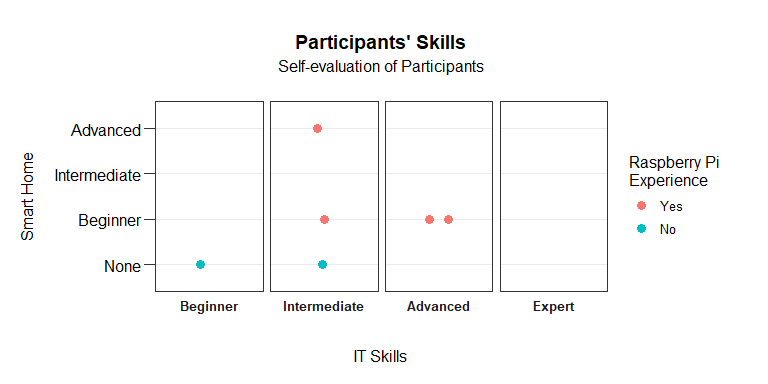
\includegraphics[width=.95\linewidth]{Bachelorarbeit/img/exp_skills.png}
    \caption{Participants categorised by their IT-Skills, Smart Home, and Raspberry PI experience}
    \label{fig:exp_skills}
\end{figure}

Overall, participants found setting up a Home Assistant instance on a Raspberry Pi to be rather easy throughout all phases of the experiment. Only one participant encountered challenges during the configuration process, which included the onboarding process and connecting devices to the instance. They stated that this was mostly due to the overwhelming user interface of Home Assistant. A breakdown of the perceived difficulty of the participants is visualised in Figure~\ref{fig:exp_difficulty}.

Furthermore, two patterns emerged when comparing the time required to complete the experiment. Participants who had used a Raspberry Pi before took around 12 minutes to perform all tasks, while those new to Raspberry Pi needed a few extra minutes. However, this was mainly due to the extra time that they needed to flash the Home Assistant image on the micro-SD card. The Raspberry Pi assembly process did not present a particularly challenging task. Further information on the time required by the participants for each phase can be found in Figure~\ref{fig:exp_timeSpent}. It should be noted that these times do not include the preparation time that is needed by the Raspberry Pi to download all dependencies from the linux package repository (up to 20 minutes) since this is idle time for the user and not relevant for this experiment

\begin{figure}[H]
    \centering
    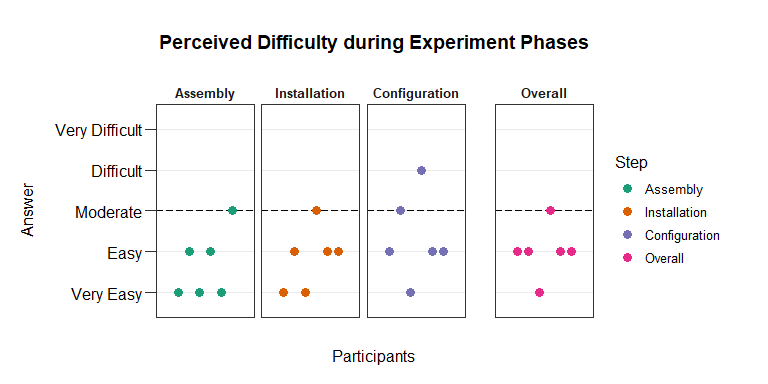
\includegraphics[width=.95\linewidth]{Bachelorarbeit/img/exp_difficulty.png}
    \caption{Perceived Difficulty of Participants during Experiment Phases}
    \label{fig:exp_difficulty}
\end{figure}

\begin{figure}[H]
    \centering
    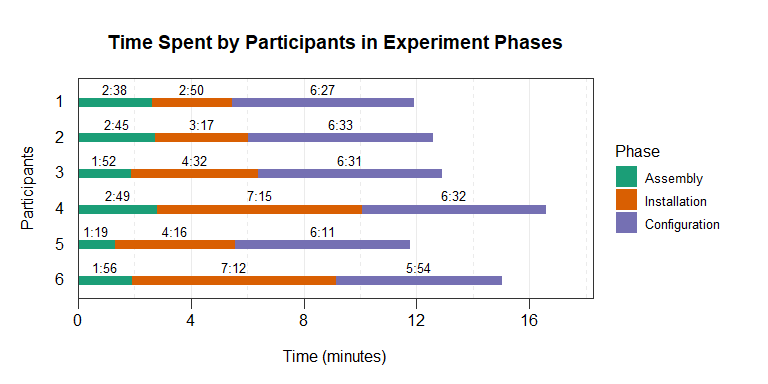
\includegraphics[width=.95\linewidth]{Bachelorarbeit/img/exp_timeSpent.png}
    \caption{Time Spent by Participants in Experiment Phases}
    \label{fig:exp_timeSpent}
\end{figure}

Although the conclusions from this experiment cannot be generalised, the results suggest that installing Home Assistant on a Raspberry PI is worth trying even for those unfamiliar with Raspberry Pi or other smart home platforms. In particular, users who already own a Pi have the opportunity to try out Home Assistant at no additional cost with a negligible investment of time and effort. Considering the confusion many participants faced when first encountering the Home Assistant user interface post-onboarding, it is recommended that new users spent some time reviewing the basic documentation pages in order to get familiar with Home Assistants' structure and features.

%% Section 7 - Conclusion

\section{Conclusion}

This paper highlighted concerns associated with the cloud-based nature of smart home technologies and devices that have been developed in the recent years which jeopardise the users' privacy and agency over their personal and smart home data. In some cases, revoking access to cloud infrastructure even renders otherwise functional devices as electronic waste. While cloud technology can be very helpful to users, the development of cloud-dependencies must be critically assessed by users who expect their devices to remain functional over many years. Home Assistant offers an alternative to this cloud-based smart home with their vision of \textit{The Open Home} that focuses on privacy, choice and sustainability through local operation and giving users full ownership of their smart home data. Additionally, this paper demonstrated that Home Assistant is a competitive alternative to traditional smart home systems, providing a wide range of advanced capabilities that allow users to enhance their smart home experience further. The only feature that Home Assistant currently cannot fully substitute is an alternative to voice assistants, where competitors still maintain an advantage due to the resource-intensive nature of voice processing. The conducted experiment suggests that any user, regardless of their technical proficiency, interested in deploying a locally hosted smart home can start using Home Assistant today on their own hardware or on power-efficient mini-computers like a Raspberry Pi.


\section*{Acknowledgements}
\addcontentsline{toc}{section}{Acknowledgements}

The author of this paper would like to sincerely thank Mr. ao.Univ.Prof. Dr.~Johann~Mitl\"ohner for his unwavering support and invaluable feedback throughout the writing of this thesis. Furthermore, the author wants to extend his thanks the open-source community, whose collective efforts help developing and improving Home Assistant and similar projects.

\newpage
% \bibliographystyle{plain}
% \bibliography{MyReferences}
\printbibliography
\addcontentsline{toc}{section}{References}

\end{document}
